% define documenclass
\documentclass[12pt, bibliography=totoc, a4paper, abstractoff, numbers=noenddot]{scrreprt}
\setcounter{secnumdepth}{3} 

% define used packages
\usepackage[left=4.0cm, right=2.0cm, top=3cm, bottom=3cm]{geometry}
%\usepackage{bibgerm}
\usepackage{babelbib}
\usepackage[utf8]{inputenc}
\usepackage[T1]{fontenc}
\usepackage{graphicx}
\usepackage[ngerman]{babel}
\usepackage{lmodern}
\usepackage{listings}
\usepackage[numbers]{natbib}
\usepackage{acronym}
\bibliographystyle{alphadin}
\usepackage{float}
\usepackage[title]{appendix}
\usepackage[table,xcdraw]{xcolor}
\usepackage{tabularx}
\usepackage{multirow}

\usepackage{lastpage}

% advanced tables
\usepackage{array}

% header and footer
\usepackage{fancyhdr}

% links
\usepackage{url}
% internal links
\usepackage[colorlinks=true ,linkcolor=black,
			anchorcolor=black ,citecolor=black ,filecolor=black,
			menucolor=black ,urlcolor=black]{hyperref}

%Makroerweiterung da urls sonst über den Rand gehen
\makeatletter 
\g@addto@macro\UrlBreaks{\do\a\do\b\do\c\do\d\do\e\do\f\do\g\do\h\do\i% 
\do\j\do\k\do\l\do\m\do\n\do\o\do\p\do\q\do\r\do\s\do\t\do\u\do\v\do\w% 
\do\x\do\y\do\z\do\&\do\1\do\2\do\3\do\4\do\5\do\6\do\7\do\8\do\9\do\0} 
\def\do@url@hyp{\do\-} 
 \g@addto@macro\UrlSpecials{\do\/{\mbox{\UrlFont/}\hskip 0pt plus 1pt}}
\makeatother
% mathematical formulas
\usepackage{amsmath, amssymb}

% fancy Diagrams %
\usepackage{tikz}
\usepackage{epstopdf}

% to include images side by side
\usepackage{subfigure}

% for nice bg on title page
\usepackage{eso-pic}
\newcommand\BackgroundPic{%
\put(0,0){%
\parbox[b][\paperheight]{\paperwidth}{%
\vfill
\centering

\includegraphics[width=\paperwidth,height=\paperheight,%
keepaspectratio]{images/Logo_H-BRS_background}%
\vfill
}}}

% define the programming language
\usepackage{listings}
\lstloadlanguages{Java,sh,bash,Haskell,HTML,PHP,XML}
\lstdefinelanguage{console}{
  morekeywords={},
  otherkeywords={warumgehtdasnicht>,\$}
}
\newcommand{\lstsetconsole}
{ \lstset{%language=sh,
        lineskip=-2pt,
        breaklines=true,
        language=console,
        breaklines=true,
        captionpos=b,
        commentstyle=\textit,
        keywordstyle=\bfseries,
        basicstyle=\ttfamily,
        stringstyle=\ttfamily,
        showstringspaces=false,
        frame=single,
        tabsize=2
  }
}
\lstdefinelanguage{scalaconsole}{
  morekeywords={},
  otherkeywords={scala>,\|}
}
\newcommand{\lstsetrepl}
{ \lstset{%language=sh,
        lineskip=-2pt,
        breaklines=true,
        language=scalaconsole,
        breaklines=true,
        commentstyle=\textit,
        keywordstyle=\bfseries,
        basicstyle=\ttfamily,
        stringstyle=\ttfamily,
        showstringspaces=false,
        frame=single,
        tabsize=2
  }
}
\newcommand{\lstsetjava}{
 \lstset{language=Java,
        breaklines=true,
        commentstyle=\textit,
        keywordstyle=\bfseries,
        basicstyle=\ttfamily,
        stringstyle=\ttfamily,
        showstringspaces=false,
        frame=single,
        captionpos=b,
        tabsize=2,
        literate=
        %linewidth=\textwidth,captionpos=b
        %numbers=left, stepnumber=5, numbersep=10pt
 }
}
\lstdefinelanguage{scala}{
  morekeywords={abstract,case,catch,class,def,%
    do,else,extends,false,final,finally,%
    for,forSome,if,implicit,import,lazy,match,mixin,%
    new,null,object,override,package,%
    private,protected,requires,return,sealed,%
    super,this,throw,trait,true,try,%
    type,val,var,while,with,yield},
  otherkeywords={_,:,=,=>,<-,<\%,<:,>:,\#,@},
  sensitive=true,
  morecomment=[l]{//},
  morecomment=[n]{/*}{*/},
  morestring=[b]",
  morestring=[b]',
  morestring=[b]"""
}
\newcommand{\lstsetscala}{
 \lstset{language=scala,
        breaklines=true,
        commentstyle=\textit,
        keywordstyle=\bfseries,
        basicstyle=\ttfamily,
        stringstyle=\ttfamily,
        showstringspaces=false,
        frame=single,
        tabsize=2
        %%linewidth=\textwidth,captionpos=b
        %numbers=left, stepnumber=5, numbersep=10pt
 }
}
\newcommand{\lstsethtml}{
 \lstset{language=HTML,
        breaklines=true,
        commentstyle=\textit,
        keywordstyle=\bfseries,
        basicstyle=\ttfamily,
        stringstyle=\ttfamily,
        showstringspaces=false,
        frame=single,
        tabsize=2
        %%linewidth=\textwidth,captionpos=b
        %numbers=left, stepnumber=5, numbersep=10pt
 }
}
\newcommand{\lstsetphp}{
 \lstset{language=PHP,
        breaklines=true,
        commentstyle=\textit,
        keywordstyle=\bfseries,
        basicstyle=\ttfamily,
        stringstyle=\ttfamily,
        showstringspaces=false,
        frame=single,
        tabsize=2
        %%linewidth=\textwidth,captionpos=b
        %numbers=left, stepnumber=5, numbersep=10pt
 }
}
\lstnewenvironment{code}
    {\lstset{}%
      \csname lst@SetFirstLabel\endcsname}
    {\csname lst@SaveFirstLabel\endcsname}
\newcommand{\lstsethaskell}{
    \lstset{
      language=Haskell,
      commentstyle=\textit,
      keywordstyle=\bfseries,
      basicstyle=\ttfamily,
      stringstyle=\ttfamily,
      showstringspaces=false,
      frame=single,
      flexiblecolumns=false,
      basewidth={0.5em,0.45em},
      literate={+}{{$+$}}1 {/}{{$/$}}1 {*}{{$*$}}1 {=}{{$=$}}1
               {==}{{$==$}}2 %{!=}{{$\not\equiv$}}2
               {>}{{$>$}}1 {<}{{$<$}}1 {\\}{{$\lambda$}}1
               {\\\\}{{\char`\\\char`\\}}1
               {->}{{$\rightarrow$} }2 {>=}{{$\geq$}}2 {<-}{{$\leftarrow$}}2
               {<=}{{$\leq$}}2 {=>}{{$\Rightarrow$} }2
               {\ .}{{$\circ$}}2 {\ .\ }{{$\circ$}}2 {(.)}{({$\circ$})}2
               {>>}{{>>}}2 {>>=}{{>>=}}2
               {|}{{$\mid$}}1
    }
}
\lstdefinelanguage{JavaScript}{
  keywords={typeof, new, true, false, catch,%
    function, return, null, catch, switch, var,%
    if, in, while, do, else, case, break},
  ndkeywords={class, export, boolean, throw, implements, import, this},
  sensitive=false,
  comment=[l]{//},
  morecomment=[s]{/*}{*/},
  morestring=[b]',
  morestring=[b]"
}
\newcommand{\lstsetjavascript}{
  \lstset{
		language=JavaScript,
		breaklines=true,
		commentstyle=\textit,
		basicstyle=\ttfamily,
		keywordstyle=\bfseries,
		stringstyle=\ttfamily,
		showstringspaces=false,
		frame=single,
		tabsize=2
  }
}
\newcommand{\lstsetxml}{
 \lstset{language=XML,
        breaklines=true,
        commentstyle=\sffamily,
        keywordstyle=\bfseries,
        basicstyle=\sffamily,
        showstringspaces=false,
        stringstyle=\ttfamily,
        frame=single,
        tabsize=2,
        literate=
        %linewidth=\textwidth,captionpos=b
        %numbers=left, stepnumber=5, numbersep=10pt
 }
}
\lstdefinelanguage{CSharp}{
 morekeywords = {abstract,event,new,struct,as,explicit,%
    null,switch,base,extern,object,this,bool,false,%
    operator,throw,break,finally,out,true,byte,fixed,%
    override,try,case,float,params,typeof,catch,for,%
    private,uint,char,foreach,protected,ulong,checked,%
    goto,public,unchecked,class,if,readonly,unsafe,%
    const,implicit,ref,ushort,continue,in,return,using,%
    decimal,int,sbyte,virtual,default,interface,sealed,%
    volatile,delegate,internal,short,void,do,is,sizeof,%
    while,double,lock,stackalloc,else,long,static,%
    enum,namespace,string,partial},
  morecomment = [l]{//},
  morecomment = [l]{///},
  morecomment = [s]{/*}{*/},
  morestring=[b]",
  sensitive = true
}
\newcommand{\lstsetcsharp}{
 \lstset{language=csharp,
        breaklines=true,
        commentstyle=\sffamily,
        basicstyle=\sffamily,
        keywordstyle=\bfseries,
        stringstyle=\ttfamily,
        showstringspaces=false,
        frame=single,
        tabsize=2
        %%linewidth=\textwidth,captionpos=b
        %numbers=left, stepnumber=5, numbersep=10pt
 }
}
\lstdefinelanguage{FSharp}{
  morekeywords={abstract,and,as,assert,base,begin,%
    class,default,delegate,do,done,downcast,downto,%
    elif,else,end,exception,extern,false,finally,for,fun,%
    function,if,in,inherit,inline,interface,internal,lazy,%
    let,match,member,module,mutable,namespace,%
    new,not,null,of,open,or,override,private,public,rec,%
    return,static,struct,then,to,true,try,type,upcast,use,%
    val,void,when,while,with,yield,asr,land,lor,lsl,lsr,lxor,%
    mod,sig,atomic,break,checked,component,const,%
    constraint,constructor,continue,eager,event,external,%
    fixed,functor,global,include,method,mixin,object,%
    parallel,process,protected,pure,sealed,tailcall,trait,virtual,volatile},     
  sensitive=false,
  morecomment=[l][\color{greencomments}]{///},
  morecomment=[l][\color{greencomments}]{//},
  morecomment=[s][\color{greencomments}]{{(*}{*)}},
  morestring=[b]"
}
\newcommand{\lstsetfsharp}{
 \lstset{language=fsharp,
        breaklines=true,
        commentstyle=\sffamily,
        basicstyle=\sffamily,
        keywordstyle=\bfseries,
        stringstyle=\ttfamily,
        showstringspaces=false,
        frame=single,
        tabsize=2
        %%linewidth=\textwidth,captionpos=b
        %numbers=left, stepnumber=5, numbersep=10pt
 }
}

%set default pagestyle
\pagestyle{empty}


\setlength{\parindent}{0pt}
\setlength{\parskip}{12pt}

% #####
% #
% # START config area
% #
% #####

\newcommand{\HEADER}[0]{H-BRS, WS 2016 / 2017}
\newcommand{\PAGENUMBERS}[0]{\pagemark}
\newcommand{\DATE}[0]{12.10.2016}
\newcommand{\AUTHOR}[0]{Eugen Besel, Johann Martens, Moritz Kemp}
\newcommand{\MATNR}[0]{}
\newcommand{\STREET}[0]{}
\newcommand{\ZIP}[0]{}
\newcommand{\TOWN}[0]{}

\newcommand{\REFERENT}[0]{Prof. Dr. Harm Knolle}
%\newcommand{\KOREFERENT}[0]{}

\newcommand{\TITLE}[0]{Aufbau einer NoSQL-Datenbank mit Apache Hadoop und Apache HBase für das Million Song Dataset}
\newcommand{\COURSE}[0]{Schemalose Datenbanken}
\newcommand{\TYPE}[0]{Semester-Projekt}
\newcommand{\COMPLETION}[0]{}

% #####
% #
% # END config area
% #
% #####

% Hurenkinder und Schusterjungenregelung
\clubpenalty=100000
\widowpenalty=100000
\displaywidowpenalty=100000

%TODO: auf Fragezeichen überprüfen
% starting the document
\begin{document}

% set pagenumbering to roman(I II III IV)
\pagenumbering{Roman}
% input the title
% #####
% #
% # This is the titlelayout from Prof. Dr. Harm Knolle 
% # (Hochschule Bonn-Rhein-Sieg)
% #  
% #####

% #####
% #
% # Default layout
% #
% #####

\AddToShipoutPicture*{\BackgroundPic}

\begin{titlepage}
  \begin{center}
  	
\includegraphics[scale=1]{./images/Logo_H-BRS.jpg}
  \end{center}
  \vspace{40pt}
  \sffamily
  \begin{tabular}{|l>{\raggedright\hspace{0pt}\arraybackslash}p{15cm}}
    & \\
    & \large\textbf{\TYPE}\\[\baselineskip]
    & \huge\textbf{\TITLE}\\[\baselineskip]
    & \textbf{Falls erforderlich: Zur Erlangung des akademischen Grades eines}\\ 
    & \COMPLETION\\
    & - \COURSE\ -\\
    & \\
  \end{tabular}
  \vfill
  \begin{tabular}{ll@{}}
    & Fachbereich Informatik\\[\baselineskip]
    &   Referent: \REFERENT\\[\baselineskip]
    &   Falls erforderlich: Korreferent: \KOREFERENT\\[\baselineskip]
    & \\[\baselineskip]
    & eingereicht von:\\[\baselineskip]
    & \AUTHOR\\[\baselineskip]
    & Matr.-Nr. \MATNR\\[\baselineskip]
    & \STREET\\[\baselineskip]
    & \ZIP \ \TOWN\\[\baselineskip]
    & \\[\baselineskip]
    & Sankt Augustin, den \DATE\\[\baselineskip]
  \end{tabular}
\end{titlepage}

%Zusammenfassung
\begin{abstract}
\section*{Zusammenfassung}\markboth{Zusammenfassung}{}
  \addcontentsline{toc}{chapter}{Zusammenfassung}
  Das Ziel der Projektarbeit zum Thema \textit{Hadoop/Hbase} ist es, 
eine Datenbank mittels Hadoop/Hbase auf einem bereitgestelltem
Cluster so zu installieren, dass der Anwender in dem One-Million-Datensatz nach Informationen zu Musikstücken
suchen kann. 


Im ersten Kapitel werden die technologischen Grundlagen zu MapReduce behandelt. Im dritten Kapitel werden das Framework Hadoop und das  NoSQL-System HBase untersucht.
Am Ende der jeweiligen Unter-Kapitel wird auch beschrieben, wie die Installation und die Konfiguration 
der Systeme abläuft. Fragestellungen werden sein, wie 
sich die Datenbank auf einen Cluster mit fünf Knoten installieren lässt und welche Konfigurationsparameter hinsichtlich des
Anwendungsfalls eines One-Million-Datensatzes berücksichtigt und angepasst werden müssen. Außerdem wird gezeigt,
ob und wie sich die Datenbank auch ohne eigens programmiertem Client Ad-Hoc ansprechen lässt, beispielsweise über
eine laufende Shell. 

Das vierte Kapitel der Projektarbeit beschreibt die praktische Umsetzung, die aus der Implementierung der Client-Software in JAVA und des Dateminports besteht.
Wichtige Fragestellungen sind dabei, inwieweit die Daten bereits für die Speicherung im Hadoop-Dateisystem geeignet sind wie die Daten auf dem Cluster-System repliziert werden.
Ebenfalls werden in diesem Kapitel die Use cases vorgestellt, die mit der Client-Software umgesetzt werden. Der Client beschränkt sich dabei auf wenige, nur funktionale Anforderungen. Eine aufwendig grafische Oberfläche ist nicht das Ziel.
Auch die konkrete Implementierung von MapReduce-Jobs wird in diesem Kapitel erläutert. 

Das letzte Kapitel beschreibt die Erfahrungen, die während des Projekts gemacht wurden, zeigt die Vor- und Nachteile auf und gibt einen Ausblick auf die Zukunft der verwendeten Technologie.

\end{abstract}


% Vorwort -TODO:Darf nicht  nicht im semesterergebnis erscheinen
% \renewcommand\abstractname{Danksagung}
\begin{abstract}
\section*{Vorwort}\markboth{Vorwort}{}
  \addcontentsline{toc}{chapter}{Vorwort}
  
% Please add the following required packages to your document preamble:
% \usepackage{graphicx}
% \usepackage[table,xcdraw]{xcolor}
% If you use beamer only pass "xcolor=table" option, i.e. \documentclass[xcolor=table]{beamer}
\begin{table}[ht!]
\centering
\resizebox{\textwidth}{!}{%
\begin{tabular}{|l|l|l|l|l|}
\hline
\rowcolor[HTML]{EFEFEF} 
Thema                                                                                                                                  & \begin{tabular}[c]{@{}l@{}}Hauptverantwortlicher\\ schriftliche Ausarbeitung\end{tabular} & \begin{tabular}[c]{@{}l@{}}Hauptverantwortlicher \\ praktische Umsetzung am Rechner\end{tabular} & \begin{tabular}[c]{@{}l@{}}Hauptverantwortlicher \\ Erstellung Vortrag\end{tabular} & \begin{tabular}[c]{@{}l@{}}Hauptverantwortlicher \\ Vortrag vorgetragen\end{tabular} \\ \hline
\begin{tabular}[c]{@{}l@{}}Ausgewählte\\ technologische Grundlagen\end{tabular}                                                        & Moritz                                                                                    & Moritz                                                                                           & Moritz                                                                              & Moritz                                                                               \\ \hline
\begin{tabular}[c]{@{}l@{}}Ausgewählte Persistenzsysteme \\ und Big Data Frameworks\\ - Vorstellung des Systems\end{tabular}           & \begin{tabular}[c]{@{}l@{}}Hadoop: Eugen\\ HBase: Johann\end{tabular}                     & -                                                                                                & Johann                                                                              & \begin{tabular}[c]{@{}l@{}}Hadoop: Eugen\\ HBase: Johann\end{tabular}                \\ \hline
\begin{tabular}[c]{@{}l@{}}Ausgewählte Persistenzsysteme \\ und Big Data Frameworks\\ - Installation des Systems\end{tabular}          & \begin{tabular}[c]{@{}l@{}}Hadoop: Moritz\\ HBase: Johann\end{tabular}                    & \begin{tabular}[c]{@{}l@{}}Hadoop: Moritz\\ HBase: Johann\end{tabular}                           & Moritz                                                                              & Moritz                                                                               \\ \hline
\begin{tabular}[c]{@{}l@{}}Ausgewählte Persistenzsysteme \\ und Big Data Frameworks\\ - Ad-Hoc-Anwendungen \\ des Systems\end{tabular} & Johann                                                                                    & Eugen                                                                                            & Johann                                                                              & Johann                                                                               \\ \hline
\begin{tabular}[c]{@{}l@{}}Ausgewählte Persistenzsysteme \\ -Implementierung der \\ Beispiel-Datenbank\end{tabular}                    & Eugen                                                                                     & Eugen                                                                                            & Johann                                                                              & Johann                                                                               \\ \hline
\begin{tabular}[c]{@{}l@{}}Ausgewählte Anwendungsszenarien\\ - Spezifikation des \\ Anwendungsszenarios\end{tabular}                   & Johann                                                                                    & \begin{tabular}[c]{@{}l@{}}HBase: Eugen\\ MapReduce-Jobs: Moritz\end{tabular}                    & Johann                                                                              & Johann                                                                               \\ \hline
\begin{tabular}[c]{@{}l@{}}Ausgewählte Anwendungsszenarien\\ - Spezifikation der konkreten \\ Anwendung\end{tabular}                   & Eugen ???                                                                                 & \begin{tabular}[c]{@{}l@{}}HBase: Eugen\\ MapReduce-Jobs: Moritz\end{tabular}                    & Eugen                                                                               & Eugen                                                                                \\ \hline
\begin{tabular}[c]{@{}l@{}}Ausgewählte Anwendungsszenarien\\ - Implementierung der Anwendung\end{tabular}                              & Eugen                                                                                     & \begin{tabular}[c]{@{}l@{}}HBase: Eugen\\ MapReduce-Jobs: Moritz\end{tabular}                    & Johann                                                                              & Eugen                                                                                \\ \hline
\end{tabular}%
}
\caption{My caption}
\label{my-label}
\end{table}
\end{abstract}


%Inhaltsverzeichnis
% loads the fancy pagestyle for register part
% set the pagestyle to fancy
\pagestyle{fancy}

\fancyhf{}% clear all fields
  % define the header
  \fancyhead[L]{\leftmark}% left header
  \fancyhead[R]{\HEADER}% right header
  \renewcommand{\headrulewidth}{0.4pt}% top line

  % define the footer
  \fancyfoot[L]{\AUTHOR}% left footer
  \fancyfoot[R]{\pagemark}% right footer
  \renewcommand{\footrulewidth}{0.6pt}% bottom line

  % redefine the chaptermark to have '1. Chaptername' and not 'CHAPTER 1.
  % CHAPTERNAME'
  \renewcommand{\chaptermark}[1]{\markboth{\thechapter.\ #1}{}}

% override the plain style
\fancypagestyle{plain}{%
\fancyhf{}% clear all fields
  % define the header
  \renewcommand{\headrulewidth}{0.0pt}% top line

  % define the footer
  \fancyfoot[L]{\AUTHOR}% left footer
  \fancyfoot[R]{\pagemark}% right footer
  \renewcommand{\footrulewidth}{0.6pt}% bottom line
}


% create the registers
\tableofcontents\newpage

% set pagenumbering to arabic(1 2 3 4)
\pagenumbering{arabic}
% loads the fancy pagestyle for main part
% set the pagestyle to fancy
\pagestyle{fancy}

\fancyhf{}% clear all fields
  % define the header
  \fancyhead[L]{\leftmark}% left header
  \fancyhead[R]{\HEADER}% right header
  \renewcommand{\headrulewidth}{0.4pt}% top line

  % define the footer
  \fancyfoot[L]{\AUTHOR}% left footer
  \fancyfoot[R]{\PAGENUMBERS}% right footer
  \renewcommand{\footrulewidth}{0.6pt}% bottom line

  % redefine the chaptermark to have '1. Chaptername' and not 'CHAPTER 1.
  % CHAPTERNAME'
  \renewcommand{\chaptermark}[1]{\markboth{\thechapter.\ #1}{}}

% override the plain style
\fancypagestyle{plain}{%
\fancyhf{}% clear all fields
  % define the header
  \renewcommand{\headrulewidth}{0pt}% top line

  % define the footer
  \fancyfoot[L]{\AUTHOR}% left footer
  \fancyfoot[R]{\PAGENUMBERS}% right footer
  \renewcommand{\footrulewidth}{0.6pt}% bottom line
}




% #####
% # load the chapter from the files
% #
% # TODO: create new chapter
% #####
\chapter{Ausgewählte technologische Grundlagen}
\section{Das MapReduce-Framework}
MapReduce wurde 2004 von zwei Mitarbeitern von Google vorgestellt \cite{dean2008mapreduce}. Es ist ein Framework
für die Entwicklung von massiver, paralleler Datenverarbeitung sehr großen Datenmengen auf Clustern.



Der Programmierer
kann sich dabei komplett auf die Verarbeitung der Daten konzentrieren. Das Framework kümmert sich um die parallele
Ausführung der Arbeit, ohne dass der Programmierer der Anwendung wissen muss, welche Daten konkret wo verteilt vorliegen
und verarbeitet werden. 
Im Zusammenarbeit mit speziellen Filesystemen 
für große Cluster-Systeme, die zum Beispiel automatisch redundante Kopien auf mehreren Maschinen anlegen, ermöglicht
eine mit MapReduce programmierte Anwendung zudem eine hohe Toleranz gegenüber dem Ausfall von einzelnen Maschinen.

\subsection{Arbeitsweise von MapReduce}
Auf der obersten Abstraktionsebene besteht das MapReduce-Framework nur aus zwei spezifizierten Funktionen: \textit{map} und \textit{reduce}.
Beide Funktionen müssen vom Anwender des MapReduce-Frameworks implementiert werden.
\textit{Map} nimmt eine, möglicherweise ungeordnete, Liste von Daten entgegen, die Schlüssel-Wert-Paare (key/value) enthält. Die Funktion 
verarbeitet nun diese Liste nach dem vom Programmierer implementierten Funktion und liefert als Ergebnis wiederum eine
Liste von Schlüssel-Wert-Paaren. Die konkrete Logik der \textit{Map}-Funktion ist vom Anwendungsfall abhängig, bildet aber in der Regel
ungeordneten Daten in eine Liste ab, die die für den Anwendungsfall interessanten Daten enthält. 


%Beispiel?
%Ein gern genommenes Beispiel
%ist das Zählen von Wörtern in tausenden von Dokumenten. Die Liste für die Eingabe in die \textit{map}-Funktion enthält für jeden Schlüssel
%als Wert ein ganzes Dokument. Diese Dokumente werden durchsucht und gleichzeitig eine neue, deutlich größere Liste mit Schlüssel-Wert-Paaren erstellt, 
%die für jedes einzelne Wort den String selbst als Schlüssel speichert, und als Wert eine 1 angibt. Somit ist jedes Wort in dieser Liste repräsentiert.
%Diese neue Liste enthält sehr viele gleiche Schlüssel, wobei alle den Wert 1 tragen.

Das Ergebnis von der \textit{Map}-Funktion ist aber nur ein Zwischen-Ergebnis und wird direkt als Eingabe für die \textit{Reduce}-Funktion verwendet,
die am Ende das tatsächliche Ergebnis der Verarbeitung ausgibt. Die \textit{Reduce}-Funktion hat in der Regel die Aufgabe, das Ergebnis der \textit{Map}-Funktion
zusammenzufassen.  

%Bezogen auf das Beispiel mit der Zählung von Wörtern bekommt die \textit{reduce}-Funktion nun eine (sehr lange) Liste von allen Wortvorkommnissen.
%Die Funktion sortiert  nun diese Liste und erzeugt eine neue Liste, die alle Schlüssel-Werte enthält, aber nur ein einziges mal in der Liste. Mehrfache Einträge
%in der ursprünglichen Liste mit gleichen Schlüsselwerten werden also zu einem Eintrag zusammengefasst, wobei die Werte der einzelne, mehrfachen Einträge
%aufaddiert werden. Das Ergebnis ist eine Liste mit jedem Wort, das in den Dokumenten vorkommt, als einmaliger Schlüssel und als Wert die jeweilige Häufigkeit.

Neben den beiden Funktionen \textit{map} und \textit{reduce} liefert das MapReuce-Framework auch eine Laufzeitumgebung mit, in der jene beiden Funktionen eingebettet sind.
Die Laufzeitumgebung kümmert sich dabei um die Verteilung der Arbeit auf dem Cluster. 
Dafür werden erstens die implementierten \textit{Map-} und \textit{Reduce}-Funktionen
kopiert und auf die einzelnen Maschinen im Cluster verteilt. Zweitens werden die Eingabedaten zerteilt und die einzelnen Daten-Stücke auf die Maschinen verteilt. 

Die konkrete Implementierung der Laufzeitumgebung hängt vom Einsatzort und Zweck ab. 
Google schlägt in seinem Paper folgendes Konstrukt vor, das in Abbildung \ref{fig:mapreduce} visualisiert wird.

\begin{figure}
\centering
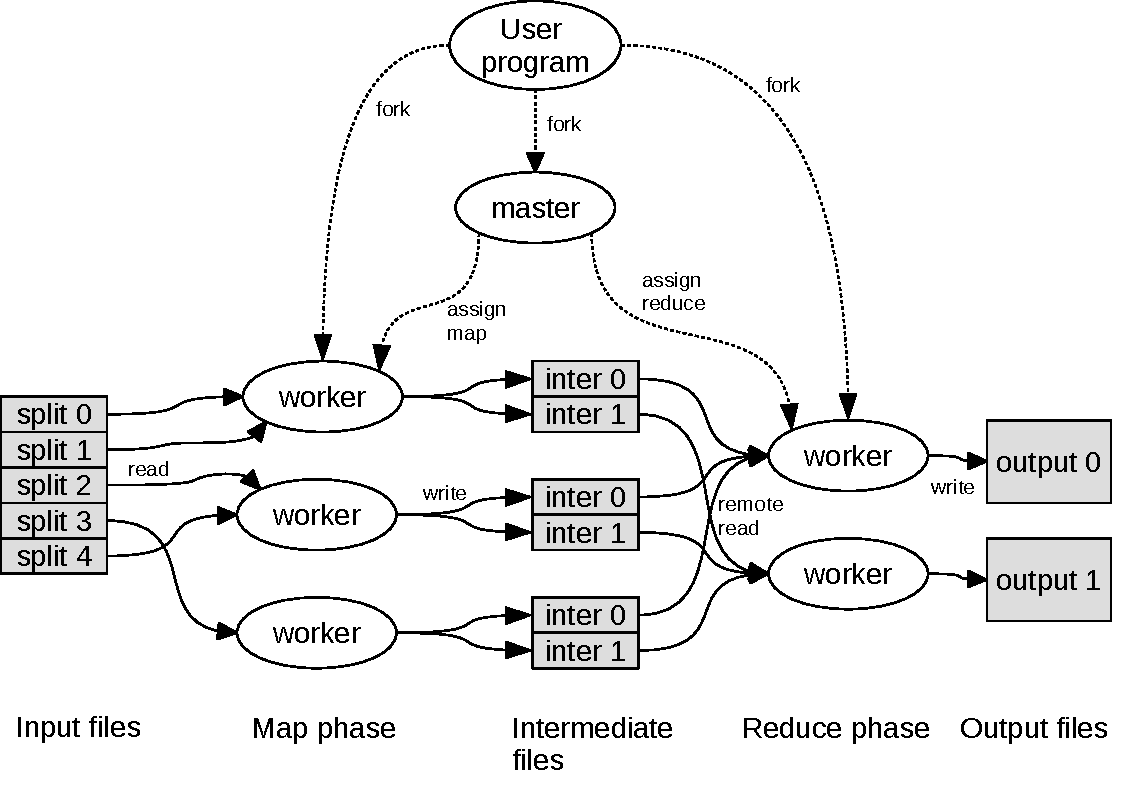
\includegraphics[width=1.0\textwidth]{images/mapreduce.pdf}
\caption{MapReduce-Laufzeitumgebung wie von Google vorgeschlagen. \cite{miner2012mapreduce}}
\label{fig:mapreduce}
\end{figure}

Die Verarbeitung von Daten mittels MapReduce läuft dann folgendermaßen ab:

Die Eingabedateien werden in $M$ gleich große Teilstücke von üblicherweise $16 MB$ bis $64 MB$
aufgeteilt. Das vom Nutzer implementierte Programm enthält die \textit{Map}- und 
\textit{Reduce}-Funktionen. Die einzelnen Maschinen (\textit{worker}) im Cluster bekommen jeweils
eine Kopie des Programms. Dabei ist eine einzige Kopie der Master, der sich anschließend
um die Koordination der Arbeit kümmert. Mit den $M$ gleich großen Teilstücken stehen nun
auch $M $ \textit{Map}-Aufgaben bereit zur Verarbeitung. Anschließend wird auch die Anzahl der Teilstücke
der Zwischenergebnisse $R$ ermittelt. Diese Anzahl $R$ stellt dann die Menge der verfügbaren
\textit{Reduce}-Aufgaben dar.

Nach dieser Vorbereitung kann die Arbeit nun schließlich beginnen. Dafür schaut der Master nach,
welche Maschinen beziehungsweise Worker nicht beschäftigt sind und weist ihnen entweder eine \textit{Map}- oder \textit{Reduce}-Aufgabe zu. Die \textit{Map}-Worker beginnen nun
die ihnen zugewiesenen Dateien zu bearbeiten, die aus Schlüssel-Wert-Paaren bestehen und
erzeugen die Zwischen-Dateien. Die Zwischen-Ergebnisse sind ebenfalls nach Schlüssel-Wert-Paaren
strukturiert. Die Zwischen-Ergebnisse werde dabei in $R$ Teil-Bereiche eingeordnet, abhängig
von ihrem Schlüssel-Wert.

Sobald ein oder mehrere \textit{Map}-Aufgaben erledigt sind, teilt der Master ein oder mehreren 
\textit{Reduce}-Workern, die gerade nichts zu tun haben, mit, dass sie mit der Verarbeitung beginnen können. Der Master teilt ihnen dabei auch mit, wo die entsprechenden Zwischenergebnisse liegen,
die sie verarbeiten sollen. Die \textit{Reduce}-Workers verarbeiten nun diese Dateien und erzeugen
mit ihrer Ausgabe einen Teil des End-Ergebnisses.


\subsection{Beispiel}
Als Beispiel dient die Analyse einer großen Datenmenge von Musiksongs mit Hilfe von MapReduce. Die Daten liegen als
Schlüssel-Wert-Paare vor. Jeder Song hat dabei einen eigenen Schlüssel, die Song-ID, sowie eine Reihe von Song-Informationen als Wert.
Die Song-Informationen beinhalten Daten wie Name des Songs, der Künstler, Beats per minute, aktueller Rank in den Charts etc.

Wir wollen nun in diesem sehr großen Datensatz an Songs herausfinden, welcher Künstler wie viele Songs geschrieben hat. Wir gehen in diesem Beispiel davon aus, dass wir eine Kenntnis davon haben, welche Künstler in  dem Datensatz vorkommen.
Im ersten Schritt müssen wir die \textit{Map}-Funktion beschreiben. Sie bekommt als Eingabe eine Reihe von Songs mit der Song-ID
als Schlüssel und ihren Eigenschaften als Werte. Diese Songs werden nun direkt auf ein Zwischenergebnis gemappt, indem der
Künstler-Name als Schlüssel und die Zahl $1$ als Wert geschrieben werden. Dies führt zu einem (großen) Zwischenergebnis,
bei dem die Anzahl der Vorkommnisse eines Künstlernames die Anzahl seiner Songs wiedergibt. Das muss aber
natürlich noch als Endergebnis zusammen gefasst werden, was dann die \textit{Reduce}-Funktion übernimmt. 

Die \textit{Reduce}-Funktion bekommt vom Master einen Werte-Bereich aus dem Zwischenergebnis zugewiesen, die sie auf
ein Endergbnis reduzieren soll. Sie holt sich dann anschließend diesen Wertebereich des Zwischenergebnisses von den verteilten
\textit{Map}-Maschinen. Sie fasst nun alle gleichen Schlüssel zu einem einzigen Schlüssel zusammen und addiert 
ihren Wert jeweils auf. Da der Wert immer $1$ ist, steht am Schluss neben dem Künstler-Name die Anzahl seiner geschriebenen
Songs. Dieses Ergebnis schreibt die  \textit{Reduce}-Funktion nun als Ergebnis raus. Die Abbildung \ref{fig:mapreduceExample} zeigt 
das Beispiel anschaulich.

\begin{figure}
\centering
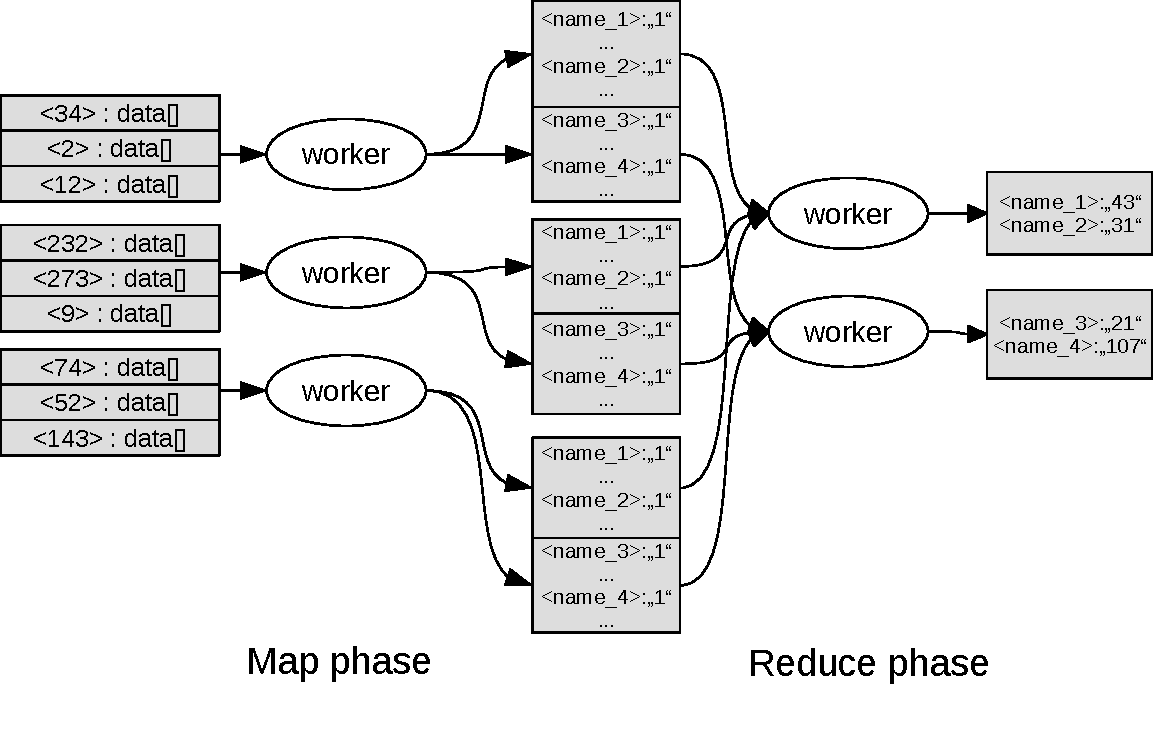
\includegraphics[width=1.0\textwidth]{images/mapreduceExample.pdf}
\caption{Ermittlung der Anzahl der Songs für jeden Künstler mittels MapReduce.}
\label{fig:mapreduceExample}
\end{figure}

%\subsection{Implementierung von MapReduce-Funktionen}

Dieser Abschnitt beschreibt die Implementierung von Map-Reduce-Funktionen, die auf den Daten
des Million-Song-Datensatzes arbeiten. Vorausgesetzt wird, dass der Million-Song-Datensatz als
CSV-Datei bereit in das HDFS-Dateisystem importiert ist. Die hier vorgestellten MapReduce-Funktionen
arbeiten ausschließlich mit Daten auf dem HDFS-Dateisystem, abgesehen von den Zwischenergebnissen,
die auf dem lokalen Dateisystem des jeweiligen Knotens abgelegt werden.



%Kein Thema in diesem Kapitel zugeordnet
\chapter{Ausgewählte Persistenzmodelle}
%\input{2.06.00}
\chapter[Ausgewählte Persistenzsysteme]{Ausgewählte Persistenzsysteme und Big Data Frameworks}
%Hadoop-Kapitel
\section{Hadoop}
%\cite{Wartal2012}
%\cite{Endlich2011}
\subsection{Visitenkarte}%alles ohne Technologie
Hadoop ist ein Java basiertes Open Source Framework von Apache. 
Die Entwicklung von Hadoop wurde als Teilpojekt von Nutch angefangen. Nutch selber ist eine Weiterentwicklung von Apache Lucene. Das Ziel des Projektes Nutch war es eine schnelle Websuche, also eine Alternative zu Google, zu entwickeln. Die Herausforderung für die Nutch Entwickler war hierbei die Erstellung eines Systems, welches mit hoch skalierbaren Prozessen, Redundanzen, automatischer Fehlerbeseitigung und Lastverteilung umgehen kann. Als Google im Jahr 2004 MapReduce und das \ac{GFS} Konzept vorgestellt hat, erkannte Doug Cutting, der Erfinder von Nutch, die Vorteile und hat sie für Nutch übernommen. Im Jahr 2006 wurde Doug Cutting von Yahoo, seinem damaligen Arbeitgeber, damit beauftragt das verteilte Dateisystem und das MapReduce-Framework aus dem Nutch-Kontext zu extrahieren und in ein eigenes Framework zu überführen. So entstand Hadoop, dessen Name von dem Spielelefanten von Doug Cuttings Sohn stammt. Im Juli 2008 gewann Hadoop den Terabyte-Sort-Benchmark, was bereits damals die Reife des entstandenen Projektes zeigte. \cite[S. 24]{Wartal2012}

Mit den neuen Konzepten von Google ermöglicht Hadoop das Verteilen der Verarbeitung komplexer Prozesse über mehrere Knoten innerhalb eines Clusters.
Die Hauptziele von Hadoop sind:

\begin{itemize}
\item Erreichbarkeit: Hadoop läuft in einem großen Cluster von Rechnern oder in einer Cloud 
\item Robustheit: Wenn ein Knoten ausfällt, übernehmen andere Knoten die Verarbeitung der Daten
\item Skalierbarkeit: Hadoop skaliert linear. Es können dynamosch weitere Rechner dazugeschaltet werden, um damit die Performance des Systems zu verbessern.
\item Einfachheit: Hadoop ermöglicht eine schnelle Entwicklung der parallelen Prozesse. %Wirklich ??
\cite{HadoopInAction}
\end{itemize}


\subsection{Systemtechnologie}% ausgewählte technologische Aspekte (Architektur, Funktionsweise, ...) ohne (ausführliche) Modellierungsaspekte
Hadoop besteht aus mehreren Modulen, die im Weiteren kurz beschrieben werden:

\begin{figure}[htbp] 
  \centering
     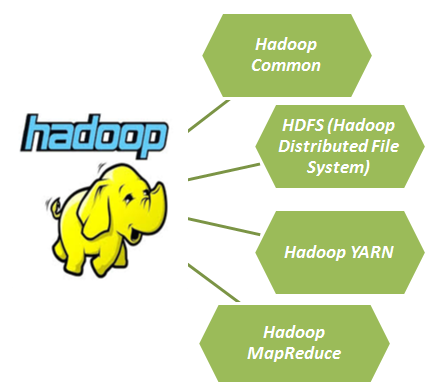
\includegraphics[width=0.5\textwidth]{images/06hadoop_modules.png}
  \caption{Hadoop-Module \cite{HaMo}}
  \label{fig: Hadoop-Module}
\end{figure}

\begin{itemize}
\item Hadoop Common: Hadoop Common stellt die Grundfunktionen bereit, die alle anderen Komponenten benötigen. Dazu zählen eine implementierungsneutrale Filesystem-Schnittstelle, die Schnittstelle für die "Remote Procedure Call"-Kommunikation im Cluster und Bibliotheken für die Serialisierung von Daten.
\item Hadoop YARN: Ein Modul für das Job-Scheduling und Cluster-Resource-Maagement
\item \ac{HDFS}: Verteiltes Dateisystem, welches einen hoch perfomanten Zugriff auf die Daten bereitstellt.
\item Hadoop MapReduce: Es ist ein auf YARN- basiertes System für die parallele Verarbeitung von riesigen Datenmenge.
\end{itemize}
Es ist möglich, Hadoop mit mehreren Dateisystemen zu betreiben: FS, HFTP FS, S3 FS etc. Das gängigste Dateisystem ist aber das \ac{HDFS}. Dieses Dateisystem basiert auf dem Google File System (\ac{GFS}). 
HDFS verwendet eine Master / Slave Architektur. Dabei verwaltet der Masterknoten (NameNode) die Metadaten von dem Dateisystem. Die Slave Knoten (DataNode) speichert die aktuellen Daten.
\subsubsection{NameNode}
Der \textit{NameNode} verwaltet alle Dateioperationen im Hadoop-Cluster. Er beinhaltet Information über die Unterteilung der Daten in Blocks und auf welcehn Knoten die Blöcke gespeichert werden.
Die Prozesse des  \textit{NameNodes} sind sehr Speicher- und I/O-lastig. Deswegen sollten \textit{NameNodes} keine Benutzerdaten speichern oder in den Berechnungsprozess eingebunden sein. Daraus resultiert, dass ein Rechner nicht gleichzeitig NameNode und DataNode sein sollte.
Zusammengefasst sind die Hauptaufgaben des NameNodes im Hadoop Dateisystem:
\begin{itemize}
\item Speicherung von Metadaten des Dateisystems im Hauptspeicher
\item Koordinierte Verteilung der einzelnen Datenblöcke
\item Überwachung der einzelnen Rechner-Knoten , um einen Ausfall schnell erkennen zu können \cite[S. XX]{Wartal2012}
\end{itemize}

Alle Daten werden in Blöcke je 64 MB aufgeteilt. Im Vergleich zu gängigen Dateisystemen ist dies eine sehr großzügige Aufteilung. Zum Beispiel unterteilt das Linux Dateisystem alle Daten in 1KB große Blöcke. Die Aufteilung in solche großen Blöcke bei Hadoop basiert auf der Notwendigkeit sehr große Mengen an Informationen zu verarbeiten. Um einen Datenblock zu verarbeiten benötigt ein \textit{NameNode} in der Regel 150Byte Arbeitsspeicher. Demnach kann ein 1GB großer Arbeitsspeicher mehr als 6 Mio Dateien und Ordner verwalten. \cite[S. XX]{Wartal2012}
\subsubsection{DataNode}
Ein \textit{DataNode}, auch Slve-Knoten genannt, ist für die Speicherung der Daten in \ac{HDFS} verantwortlich. Er berichtet dem \textit{NameNode} über den Status der Datenverarbeitung in regelmäßigen Abständen und meldet sich bei seinem Start bei ihm an. Die Daten werden auf mehrere \textit{DataNodes} repliziert, um die Ausfallsicherheit gewährleisten zu können.
Ein\textit{DataNode} benötigt sehr viel Speicherkapazität, weil alle Daten ihm gespeichert sind \cite{nameNode}.


\subsubsection{Secondary NameNode}
Um die Aufgabe eines Secondary Nodes zu verstehen betrachten wir ganz kurz welche Dateien von einem NameNode geschrieben werden und welche Probleme dabei entstehen:
\begin{figure}
	\centering
	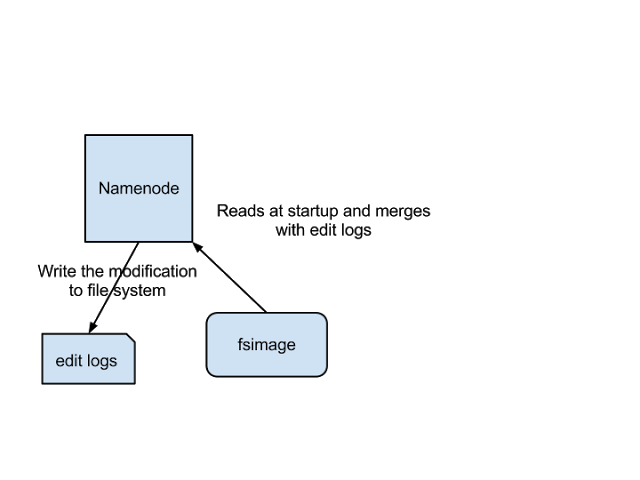
\includegraphics[width=1.0\textwidth]{images/namenode.png}
	\caption{NameNode}
	\label{img:grafik-nameNode}
\end{figure}

Wie aus der Abbildung zu sehen ist, schreibt ein NameNode zwei unterschiedliche Dateien auf die Festplatte. \\
\begin{itemize}
\item FsImage ist eine Momentane Aufnahme des Dateisystem zum Zeitpunkt des Starts des NameNodes
\item Edit Logs beinhaltet eine Menge der Änderungen, die nach dem Starten eines NameNodes auftreten.
\end{itemize}
Ein FsImage wird nur beim Neustart eines NameNodes geschrieben. Dabei wird die Information aus dem EditLog in den FsLog geschrieben um die momentane Aufnahme des Dateisystems zu speichern.\\
Da in der Regel ein NameNode sehr selten neu gestartet wird, entstehen folgende Probleme:
\begin{itemize}
\item EditLog wird sehr groß und kann nicht verwaltet werden.
\item Das Neustarten eines NameNode dauert auf Grund der großen Datenmenge sehr lange.
\item Im Fall eines Ausfalls des NameNodes geht sehr große Menge an Information verloren.
\end{itemize}
Secondary NameNode wird dafür benötigt um die oben beschriebenen Probleme zu umgehen.\\
\begin{figure}
	\centering
	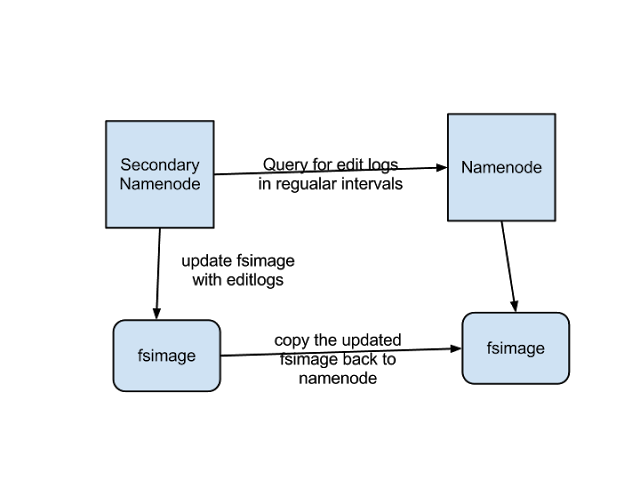
\includegraphics[width=1.0\textwidth]{images/secondarynamenode.png}
	\caption{SecondaryNameNode}
	\label{img:grafik-SecondaryNameNode}
\end{figure}
Aufgaben eines Secondary NameNodes sind:
\begin{itemize}
\item Ein Secondary NameNode holt in der regelmäßigen Abständen die Daten aus dem EditLog und verschiebt sie in den FsImage.
\item Sobald ein neuer FsImage vorhanden ist, wird es auf den NameNode geschrieben.
\item 3. Der neue FsImage wird beim nächsten Neustart des NameNodes verwendet, was die Zeit des Prozess stark reduziert.
\end{itemize}
\cite{secNameNode}

\subsubsection{Replikation der Daten in Hadoop}
Hadoop verwendet einen blockorientierten Ansatz für die Datenreplikation. Mit dem Ansatz wird jede im HDFS abgelegte Datei in einzelne Blöcke mit einer festen Bytegröße aufgeteilt und durch den NameNode auf unterschiedliche Clusterknoten abgelegt. Zusätzlich wird durch den NameNode sichergestellt, dass jeder Block mehrfach auf unterschiedliche Knoten im Cluster repliziert wird.
In der HDFS-Standardkonfiguration repliziert der NameNode jeden Block dreifach. Kommt es nun zum Ausfall eines Knotens im Cluster, gehen nur die auf dem ausgefallenen Rechners sich befindlichen Blöcke verloren und keine ganze Datei, da die verloren gegangenen Blöcke durch ihre Kopien auf anderen Knoten ersetzbar sind und so der NameNode die ganze Datei bereitstellen kann.
\cite{replikation}

\subsection{Datenmodell}
In diesem Projekt wird im Bezug auf Datenmodellierung lediglich das \ac{HDFS} aus dem Hadoop-Framework genutzt. 

\subsection{Systeminstallation} % Installation auf der Grundlage unseres Clusters
Da Hadoop in Java implementiert ist, ist es Platformunabhängig und kann sowohl auf Windows, Linux oder MacOs installiert werden.
Im Folgenden Kapitel wird beschrieben, wie man Hadoop auf mehreren Knotten installieren kann. 

Bevor man mit der Installation des Hadoop System begint, müssen zwei Voraussetzungen erfüllt werden.
1. Die Grundlage für eine lauffähige Hadoop Instanz ist eine Java Laufzeitumgebung. Für Hadoop braucht man mind. Java Version 1.6.
Nachdem Java auf der dafür vorgesehenen Maschine installiert ist, muss man die JAVA\_HOME auf das richtige Java Verzeichnis setzen.\\
2. SSH muss installiert werden und sshd muss laufen, damit die Hadoop Scripte ausgeführt werden können.\\
Nachdem die Voraussetzungen erfüllt sind, kann man mit der Installation von Hadoop beginen. Diese beinhaltet das Laden einer Hadoop Distribution aus dem Internet und die Konfiguration dieser für ein Single- bzw ein MultipleMode. Bei einer Cluster Installation muss Hadoop auf jeden Knoten des Clusters abgelegt werden.
Man kann Hadoop auf der Seite von Apache Hadoop  (http://hadoop.apache.org/releases.html) laden.\\
Die Konfiguration von Hadoop wird auf zwei Arten von Dateien verteilt:
\begin{itemize}
\item Read-only default configuration - core-default.xml, hdfs-default.xml, yarn-default.xml and mapred-default.xml.
\item Site-specific configuration - etc/hadoop/core-site.xml, etc/hadoop/hdfs-site.xml, etc/hadoop/yarn-site.xml and etc/hadoop/mapred-site.xml.
\end{itemize}
\cite{hadoopConfiguration}


Sämtliche Konfigurationsdateien befinden sich in der Hadoop Version 2.7.3 im folgenden Verzeichnis: etc/hadoop/
Als erstes betrachten wir die Konfigurationdatei hadoop-env. In dieser Datei findet man einen Hinweis auf die installierte Java Version, spezifischen Speichereinstellugen usw. 
Eine weitere wichtige Konfigurationsdatei core-site.xml beinhaltet das Verzeichnis und die Adresse des Hadoop-Dateisystems. Bei der frischen Hadoop Installation ist diese Datei leer und muss mit Inhalt befüllt werden.
Der Parameter hadoop.tmp.dir legt fest, in welchem Verzeichnis Hadoop die benötigten Dateien für das HDFS anlegen darf.

Der Parameter fs.defaultFS beschreibt die URI von dem NameNode

Eine weitere Konfigurationsdatei hdfs-site.xml bestimmt unter anderem den Grad der Replikation innerhalb der HDFS an.
Darüber hinaus kann man in dieser Datei den Pfad zum Verzeichnis finden, in dem die Daten von dem NameNode (dfs.namenode.name.dir) oder aber die Daten von dem DataNode(dfs.datanode.data.dir) liegen.

Die vollständige Liste aller Konfigurationsparameter inklusive ihrer Default-Werte finden sich unter:

\begin{itemize}
	\item \url{https://hadoop.apache.org/docs/r2.7.2/hadoop-project-dist/hadoop-common/core-default.xml}
	\item \url{http://hadoop.apache.org/docs/r2.7.2/hadoop-project-dist/hadoop-hdfs/hdfs-default.xml}
	\item \url{https://hadoop.apache.org/docs/r2.7.2/hadoop-yarn/hadoop-yarn-common/yarn-default.xml}
\end{itemize}

\subsection{Datenschema}
Das logische Datenschema wird in Abschnitt \ref{hbase_datenschema}  beschrieben.

\subsection{Ad-Hoc-Zugriffsmöglichkeiten}
CRUD-Operationen können in Hadoop auch ohne HBase über einen Hive-Client durchgeführt werden. Dies war jedoch nicht Bestandteil dieses Projekts. CRUD-Operationen mit HBase werden in Abschnitt \ref{hbase_adhoc} beschrieben.

\newpage
%HBase-Kapitel
\section{HBase}

%\cite{Redt01} embeddeed in text.
%\cite{SpaOd16} embeddeed in text.


Im Folgenden wird HBase als \textbf{die} Hadoop Datenbank vorgestellt, die zu Grunde liegende Systemtechnologie erläutert  und die Installation/Konfiguration beschrieben.
\subsection{Visitenkarte}
\subsubsection{Entstehung}
Nachdem Google immer größer werdende Datenmassen speichern musste und dieses Problem mit dem  \ac{GFS} gelöst zu sein schien, stellten sich weitere Probleme heraus: 
Die Indexierung dieser Daten und die Verteilung der Daten auf viele Knoten ohne Zugriffgeschwindigkeit und Konsistenz zu verlieren. Google fand eine Lösung mit BigTable und auf Grundlage des veröffentlichten WhitePapers \cite{bigtable} dazu, entwickelte die Open-Source-Community dann HBase. Aus diesem Grund weisen diese beiden Datenbanken auch Gemeinsamkeiten bezüglich ihrer Funktionalität auf. Beispielsweise unterstützen beide die Komprimierung (siehe \ref{tableoperation}) und Versionierung der Daten \cite{SpaOd16}.

\subsubsection{Allgemein}
HBase wurde entwickelt, um mit Hadoop zusammen zu arbeiten, ist ein verteiltes BigData-Speichersystem 
 und bietet einen schnellen (nahe Echtzeit) Zugriff auf riesige Datenmengen.

%Bei unvollständigen Datensätzen, im Relationalen Sinne gesprochen, bei Einträgen mit fehlenden Attributen und einem sich oft wechselndem Schema empfiehlt sich der Einsatz von HBase.
%speicherbasierte Tabellen
%Bietet geringe Latenz bei Zugriff auf kleine Teil-Datenmengen 
%Bietet ein flexibles Datenmodel
%build for low latency querries
%Ein verteiltes Speichersystem für strukturierte Daten

%Key-value
%value wird von einem Key identifiziert
%Key und value sind beide byte-array
%Werte können schnell durch die Schlüssel zugegriffen werden

\subsubsection{Portfolio}
HBase wird von vielen bekannten Konzernen eingesetzt, da es sich gut für Logging- und Suchsysteme  eignet und als Grundpfeiler für \ac{OLAP}-Systeme geeignet ist \cite{Redt01}.

\begin{figure}[H] 
  \centering
     \includegraphics[width=0.7\textwidth]{images/{06.portfolio}.png}
  \caption{HBase-Portfolio \cite{youportf}}
  \label{fig:Portfolio}
\end{figure}

%------------------------------------------------------------------------------------------------------------------------------------------------------------------------------------------------------------------------------------------------

\subsection{Systemtechnologie} % ausgewählte technologische Aspekte (Architektur, Funktionsweise, ...) ohne (ausführliche) Modellierungsaspekte
 In HBase lassen sich riesige Datenmengen auf mehreren Knoten verteilen, verwalten und jederzeit erweitern. HBase basiert auf Java, ist Open-Source, nicht-relational, spaltenorientiert und setzt auf ein verteiltes Dateisystem wie \ac{HDFS} von Hadoop auf \cite{hbasetut}. HBase, als Key-Value-Store, wurde als fehlertolerantes System entworfen, das auch gut mit unvollständige Datenmengen umgehen kann. Aufgrund des schemalosen Datenmodells, müssen nicht alle Felder belegt werden und verbrauchen auch keinen Speicherplatz \cite{compWo}.  Durch das \ac{WAL} und eine verteilte Konfiguration kann sich HBase schnell von Serverausfällen erholen \cite{Redt01}. 
 
 Nach CAP-Theorem legt es besonders Wert auf Verfügbarkeit und Partitionierung und vernachlässigt die Konsistenz der Daten.%nochmal überdenken
Des weiteren unterstützt HBase die Replikation von Hadoop, den MapReduce-Algorithmus, automatische Verteilung der Tabellen auf die Knoten, Komprimierung der Daten und Bloom-Filter. HBase kann im Standalone-Modus, im pseudo-verteilten Modus und im vollständig-verteilten Modus betrieben werden. Für den vorliegenden Usecase wird am Ende des Kapitels die Konfiguration für den vollständig-verteilten Modus beschrieben. Für diesen Modus wird für die verteilte Konfiguration ein Zookeeper benötigt (siehe Abschnitt \ref{zook}). HBase stellt zwar selbst keine SQL-API zur Verfügung lässt sich aber durch Schnittstellen wie Apache Phoenix um eben solche erweitern.

\subsubsection{Hbase im Vergleich zu einem \ac{RDBMS}}
HBase erinnert an eine relationale Datenbank, da die Daten in Tabellen gespeichert werden, die Zellen enthalten. Jedoch verhalten sich die Tabellen nicht wie Relationen und die Zeilen nicht wie Datensätze in relationalen Datenbanken. Auch sind die Spalten nicht durch ein Schema definiert.
HBase speichert die teils unvollständigen Daten in Spalten ab im Vergleich zu vollständigen Reiheneinträgen in einem \ac{RDBMS}. Dies ist notwendig da große Datenmengen den Anforderungen auf Vollständigkeit, wie sie ein \ac{RDBMS} erfordert, oftmals nicht gerecht werden.  
Während in einem \ac{RDBMS} viele schmale, normalisierte Tabellen vorliegen, ist HBase für Tabellen mit Millionen von nicht-normalisierrten Spalten ausgelegt. Die Partitionierung wird bei HBase automatisch vogenommen, währenddessen in einem RDBMS dies manuell erfolgen muss \cite{youintr}. Durch die Spaltenorientierung ist
HBase besonders gut für analytische Aufgaben geeignet, da es selectiv nur die benötigten Daten abfragt und nicht die komplette Zeile, wie es ein \ac{RDBMS} tut.


\subsubsection{HBase im Vergleich zu HDFS}
Da HBase selbst seine Daten nicht speichern kann, bedient es sich der \ac{HDFS}-Funktionen (siehe Abschnitt \ref{hadooptech}). Im Unterschied zu normalen Dateisystemen wie ext4 oder NTFS kümmert  sich \ac{HDFS} automatisch um die Replikation von Daten zwischen den Knoten,  
sodass eine hohe Skalierbarkeit und eine hohe Ausfallsicherheit entsteht. Da HDFS ein Filesystem ist, fehlt ihm die zufällige Lese-und Schreibfähigkeit. Eine mögliche Lösung dafür ist HBase. Es stellt innerhalb des Clusters in Echtzeit Lese- und Schreibzugriff zu den Daten her. Zur Speicherung großer Binärdaten ist die direkte Nutzung von HDFS besser geeignet \cite{compWo}. 
Es wird empfohlen HBase in einem verteilten System ab fünf Knoten einzusetzen \cite{SpaOd16}.

\begin{figure}[H] 
  \centering
     \includegraphics[width=0.7\textwidth]{images/{06.architecture}.png}
  \caption{HBase-Architektur \cite{clo11}}
  \label{fig:architecture}
\end{figure}


\subsubsection{MasterServer}
HBase besitzt zwei Rollen: den HBase \textit{MasterServer} und die \textit{RegionServer}. Der \textit{MasterServer} ist verantwortlich für die Zuweisung der Regionen (siehe Abschnitt \ref{region}) an die \textit{RegionServer}, die Verteilung der Last (Abschnitt \ref{tableoperation}), den Neustart der \textit{RegionServer}, die Teilung (Abschnitt \ref{tableoperation}) und die Überwachung der \textit{RegionServer}. Es ist möglich mehrere \textit{MasterServer} in einem Cluster zu betreiben, wobei aber nur einer aktiv sein kann. Da der \textit{MasterServer} nur verwaltende Funktionen inne hält, kann ein Cluster auch ohne ihn arbeiten, solange kein \textit{RegionServer} ausfällt. Spätestens dann muss ein \textit{MasterServer} eingreifen und die Regionen neu zuweisen. Die Verfügbarkeit des \textit{MasterServers} wird vom Zookeeper verwaltet \cite{Redt01}.

\subsubsection{RegionServer}
Der \textit{RegionServer} beinhaltet die HBase Regionen (siehe \ref{region}) und die HBase-Daten, welche lexikographisch nach dem Reihenschlüssel sortiert  werden. Die Aufrufe der JAVA-API gehen direkt an die \textit{RegionServer}, damit der \textit{MasterServer} nicht als Flaschenhals agiert. Der \textit{RegionServer} komprimiert und verteilt die Daten und berichtet dem  \textit{MasterServer}. Es wird empfohlen nur einen \textit{RegionServer} pro Maschine zu betreiben \cite{Redt01}. Für Lese-und Schreibzugriffe kommuniziert der \textit{RegionServer} mit anderen \textit{RegionServern}.

\begin{figure}[H] 
  \centering
     \includegraphics[width=0.9\textwidth]{images/{06.cluster}.png}
  \caption{Exemplarische Aufteilung der Tabelle in Regionen}
  \label{fig:cluster}
\end{figure}


%------------------------------------------------------------------------------------------------------------------------------------------------------------------------------------------------------------------------------------------------

\subsection{Datenmodell} %Modellierungsaspekte

\subsubsection{Tabellen}
HBase speichert die Daten, ähnlich wie eine relationale Datenbank in Tabellen. Jedoch bestehen diese aus Reihenschlüsseln und Spaltenfamilien (siehe \ref{sf}). Es gibt zwei Arten von Tabellen: Die Benutzer-Tabellen und die System-Tabellen.
Die Systemtabellen werden für das Verwalten von Meta-Daten von \acp{ACL}, Tabellen, Regionen (siehe \ref{region}) und Namensräumen verwendet. Die Benutzer-Tabellen werden im vorliegenden Projekt für die Verwaltung des Million-Song-Dataset verwendet. Folgend ein Beispiel einer solchen Tabelle:

\begin{figure}[htbp] 
  \centering
     \includegraphics[width=0.7\textwidth]{images/{06.logisch}.pdf}
  \caption{Logische Darstellung der Daten}
  \label{fig:Logische Darstellung der Daten}
\end{figure}

%Tablellen sind nach Reihen-schlüssel sortiert


\subsubsection{Regionen}\label{region}
Eine Tabelle besteht aus Spalten und Reihen. Für die Skalierung  und den randomisierten Zugriff, teilt HBase die Tabelle horizontal in Regionen auf, d.h. jede Region besteht aus einer Reihe von aufeinander folgenden Schlüsseln. Jede Region wird einem \textit{RegionServer} zugeordnet. Der HBase LoadBalancer sorgt dafür, dass die Regionen auf alle \textit{RegionServer} gleich verteilt werden. Jede Region wird durch einen Start-Schlüssel und einen End-Schlüssel begrenzt. Diese Informationen lassen sich in den System-Tabellen wiederfinden. Regionen können geteilt werden, wenn sie zu groß werden oder zusammengelegt werden, wenn die zu klein sind.

\subsubsection{Spaltenfamilien}\label{sf}
Die Empfehlung ist, dass Daten mit gleichen Zugriffs-Queries und dem selben Format in einer Spaltenfamilie zusammengefasst werden sollten. Wenn wir beispielsweise zu allen Songs des One-Million-Song-Datasets die Coverbilder der Songs hinterlegt hätten, könnten die Bilder in einer Spaltenfamilie und die textuellen Informationen zu den Songs in einer anderen Spaltenfamilie hinterlegt werden. So könnte die Spaltenfamilie mit den textuellen Informationen komprimiert werden (siehe Abschnitt \ref{tableoperation}). Wenn bestimmte Daten nur gelesen werden und andere meistens geschrieben werden, sollte ebenfalls über eine separate Spaltenfamilie nachgedacht werden. Es gibt keine Grenze nach oben für die Spaltenfamilien innerhalb einer Tabelle, jedoch leidet die Performanz bei vielen Spaltenfamilien. Der \textit{MemStore} (siehe \ref{memstore} wird dadurch belastet und generiert viele kleine Dateien. Bei der Tabellenerzeugung  muss bis auf die Spaltenfamilien keine feste Vorgabe gemacht werden. Alles außer der Tabellenname wird als Byte-Array abgespeichert, d.h. man kann Zeichen, Zahlen, Buchstaben usw. abspeichern. Um auf einen Wert zugreifen zu können, muss der Reihenschlüssel, die Spaltenfamilie, der Spaltenname und  Zeitstempel (optional) angegeben werden \cite{SpaOd16}. In der folgenden Abbildung ist zu sehen, wie HBase seine Daten abspeichert:

\begin{figure}[H] 
  \centering
     \includegraphics[width=0.9\textwidth]{images/{06.physisch}.pdf}
  \caption{Physische Darstellung einer Tabelle}
  \label{fig:Physische Darstellung einer Tabelle}
\end{figure}

\subsubsection{Spalten}
Spalten werden nicht durch eine Schema-Beschreibung vorgegeben und können jederzeit zu einer Spaltenfamilie hinzugefügt werden. Jede Spalte kann mehrere Versionen (Abschnitt \ref{versionen}) erhalten. 

\subsubsection{Stores}
Es gibt einen Store pro Spaltenfamilie. Ein Store gruppiert den \textit{MemStore} und \textbf{0-n} \textit{Store}-Files (HFiles). 

\subsubsection{MemStore}\label{memstore}
Wenn Daten hinzugefügt oder geändert werden, wird ein \ac{WAL} erzeugt und in den \textit{MemStore} geschrieben, wo der Eintrag lexikographisch einsortiert wird. Ist der Im-Memory Speicher des \textit{MemStore} voll, werden die Daten als HFile im \ac{HDFS} abgespeichert. Die Logdateien im \textit{MemStore} werden erst gelöscht, wenn alle Änderungen festgeschrieben wurden. So wird sichergestellt, dass die Daten nicht verloren gehen, falls ein Knoten abstürzt.

\subsubsection{HFiles}
HFiles (Key-Value-Map) werden erzeugt, wenn die \textit{MemStores} voll sind und werden im HDFS abgespeichert, um von der Hadoop-Persistierung und Replikation zu profitieren. HFiles bestehen aus Blöcken. Ein Block hat eine Größe zwischen 8KB und 1 MB. Die Blockgröße kann konfiguriert werden.  Die Standard-Größe liegt bei 64KB. Es gibt viele Blocktypen die innerhalb eines HFiles vorkommen können: Der Datenblock enthält sowohl die Daten als auch die \textit{Put- und Delete-Markierungen}. Indexblocks ermöglichen das schnelle Auffinden einer Reihe innerhalb eines HFiles. Bloom-Filter-Blocks werden für das Überspringen von  bestimmten Parse-Vorgängen genutzt, damit der angefragte Schlüssel schneller gefunden werden kann. Trailer Blocks enthalten die HFile-Version. 
%HFiles sind unveränderlich, da HDFS kein Update erlaubt.
Zusammenfassende eine Darstellung der HBase-Architektur:

\begin{figure}[H] 
  \centering
     \includegraphics[width=1\textwidth]{images/{06.regionserverinternals}.png}
  \caption{RegionServer-Interna \cite{carmc}}
  \label{fig:Internals}
\end{figure}

\subsubsection{Interne Tabellenoperationen }\label{tableoperation}
Die große Stärke von HBase ist es, Daten zu größeren Dateien zusammenzufassen und Tabellen automatisch auf mehrere Rechner zu verteilen. Hierzu verwendet HBase drei verschiedene Mechanismen.
\begin{description}
\item[Komprimierung]
 Um zu vermeiden, dass beim \textit{Memstore-Flush} (siehe \ref{memstore}) viele kleine HFiles entstehen, legt HBase sie zu größeren Dateien zusammen.  Alle Dateien mit dem gleichen Schlüssel, aber einem älteren Zeitstempel werden so gelöscht. Beim Löschen von Zellen setzt HBase einen Marker, der bei der Komprimierung überprüft wird. In einer weiteren Stufe der Komprimierung können alle Marker gelöscht werden. Eine solche Komprimierung kann manuell für eine spezifische Region oder Tabelle angestoßen werden. Außerdem werden standardmäßig wöchentlich solche Komprimierungen von HBase selbst ausgeführt \cite{SpaOd16}.

\item[Teilung]
Das Gegenteil der Komprimierung ist die Teilung (Split), auch \textit{Auto-Sharding} genannt. Wenn eine Region eine Größe von 10GB erreicht, führt HBase eine Teilung durch und es entstehen zwei neue Regionen. Hierbei ist zu beachten, dass Teilungen immer spaltenfamilienübergreifend stattfinden \cite{SpaOd16}:

\begin{figure}[H] 
  \centering
     \includegraphics[width=0.7\textwidth]{images/{06.split}.pdf}
  \caption{Zwei Spaltenfamilien vor und nach der Teilung}
  \label{fig:Teilung}
\end{figure}


\item[Verteilung der Last]
Eine Verteilung der Last ist insbesondere bei der Neuordnung von Daten (Komprimierung) oder der Veränderung der Cluster-Umgebung (neuer oder gelöschter Rechnerknoten) notwendig.
%Da Regionen geteilt und verdichtet werden, neue Server hinzukommen oder herunterfahren ist eine Balancierung der Last notwendig.
HBase, um genau zu sein Hadoop, führt alle fünf Minuten einen LoadBalancer aus der algorithmisch sicherstellt, dass alle \textit{RegionServer} eine ähnliche Anzahl an Regionen bedienen \cite{SpaOd16}. 
\end{description}

 \subsubsection{Versionierung}\label{versionen}
Eine Reihe, eine Spalte und ein Zeitstempel spezifizieren exakt eine Zelle in HBase. Während Spalten und Reihen gleich bleiben können, ändert sich der Zeitstempel für jede Zelle. Der Zeitstempel, als Long-Integer-Datentyp, wird in absteigender Reihenfolge hinterlegt, sodass immer der aktuellste Wert aus den HFiles gelesen wird \cite{reference}.


\subsubsection{Zugriff auf HBase}
Obwohl aus Perfomanzgründen empfohlen wird die JAVA-API für den Zugriff auf HBase zu nutzen \cite{clo11}, werden im folgenden weitere Möglichkeiten vorgestellt.
\begin{description}
\item[Thrift Server]
Der Thrift Server kann als Gateway benutzt werden, um Applikationen  anderer Sprachen, den Zugriff auf HBase zu ermöglichen. Ein C/C++ Client könnte bei dieser Lösung jedoch nur mit dem Thrift Server kommunizieren und nicht direkt auf einen \textit{RegionServer} zugreifen.

\item[REST Server]
HBase stellt auch eine REST-API zur Verfügung, auf die über HTTP zugegriffen werden kann.

\item[Hive]
\end{description}

%------------------------------------------------------------------------------------------------------------------------------------------------------------------------------------------------------------------------------------------------

\subsection{Systeminstallation} %Installation auf der Grundlage unseres Clusters 
Für die Installation werden sowohl auf dem  \textit{MasterServer} als auch auf den \textit{RegionServern} folgende UNIX-Kommandos abgesetzt:
\noindent 
\begin{lstlisting}[language=bash]
  $ wget http://www-us.apache.org/dist/hbase/stable/
    hbase-1.2.4-bin.tar.gz
  $ tar -xzf hbase-1.2.4-bin.tar.gz
  $ ln -s hbase-1.2.4 hbase
  $ cd hbase
  $ export PATH=$PATH:~/hbase/bin
\end{lstlisting}

Die Konfiguration für HBase wird in einer Datei namens \textit{hbase-site.xml} erstellt. Hier werden Zookeeper-Einstellungen vorgenommen, das HDFS-System referenziert und der Betriebsmodus sowie der Pfad zur Datenspeicherung eingestellt.
Um HBase zu starten, wird der Befehl 
\noindent 
\begin{lstlisting}[language=bash]
  $ {HBASE_HOME}/bin/start-hbase.sh 
\end{lstlisting}
ausgeführt. HBase lässt sich mit dem Standard-Port 16010 über folgende \ac{URL} über die Weboberfläche aufrufen: \textit{localhost:16010}

\subsubsection{ZooKeeper}\label{zook}
ZooKeeper ist ein Open-Source-Projekt unter der Apache-Foundation. ZooKeeper wird auf den Knoten von Clustern installiert und bietet 
Dienste für typischen Aufgaben an, die bei verteilten Anwendungen auf Clustern anfallen. Typische Probleme sind dabei Race-Conditions 
beim verteilten Schreiben auf den selben Daten, der Zugriff auf schon veraltete Daten oder überhaupt das Auffinden von den Rechnerknoten im
Cluster. ZooKeeper überwacht auch die einzelnen Knoten im Cluster durch sogenannte \textit{Heartbeats}. Dies sind kurze Signale an den  \textit{MasterServer},
die signalisieren, dass der Rechnerknoten noch aktiv ist. 

Die Installation von ZooKeeper ist verhältnismäßig einfach. Nachdem die Anwendung auf die einzelnen Knoten herunter geladen ist, muss in der 
\newline \texttt{zookeeper/conf/zoo.cfg}
die Konfiguration erfolgen, die im einfachsten Falle nur aus der Angabe der Rechner-Knoten besteht. Innerhalb von ZooKeeper nennt sich so ein Verbund
von Rechner-Knoten ein \textit{esemble}. Diese Konfiguration muss anschließend auf alle Knoten verteilt werden. Danach kann der ZooKeeper-Server, genannt \texttt{zkServer},
auf jedem Knoten manuell gestartet werden. Über den Client-Port von ZooKeeper, der in diesem Projekt auf jedem Knoten der Port $2186$ ist, können die verteilten
Anwendungen die ZooKeeper-API verwenden. Dabei können sie sogenannte \textit{zNodes} anlegen. Das sind Dateien, auf die verteilt zugegriffen wird und um dessen
Gültigkeit sich nun ZooKeeper kümmert, sodass die verteilte Anwendung sich nicht mehr um die typischen Probleme, die in einem Cluster auftauchen, kümmern muss.

\subsection{Datenschema}\label{hbase_datenschema}
Die Zeilen haben einen eindeutigen Schlüssel (RowKey) -> Zugriff auf die eigentlichen Spalten
Werte werden in Spalten versioniert (max 3 Versionen)
Spaltenfamilie wird in Regionen aufgeteilt und auf die RegionServer verteilt
Zeitstempel: Per Default wird der aktuellste Wert genommen (Beispiel: Welche User haben sich gestern eingeloggt)
Zuordnung einer Region zu genau einem Server (strikte Konsistenz) -> alle Modifikation (put und delete auf einem Server)
Atomare Operationen: Alte oder neue Werte lesen

Zusatzinfo: Alle Spalten in einer Spaltenfamilie werden in der gleichen Datei gespeichert, den sogenannten HFile-Dateien
\subsection{Ad-Hoc-Zugriffsmöglichkeiten}\label{hbase_adhoc}
%List 
%scan 'music' ,{'LIMIT' => 5}
%put 'music', 'TestRowKey', 'song:ArtistName','Team6_Test'
%get 'music', 'TestRowKey'
%Update (put 'music', 'TestRowKey', 'song:ArtistName', 'NewValue')
%Delete (deleteall 'music', 'TestRowKey')
%
%scan 'music', { FILTER => SingleColumnValueFilter.new(Bytes.toBytes('song'), Bytes.toBytes('ArtistName'), CompareFilter::CompareOp.valueOf('EQUAL'),BinaryComparator.new(Bytes.toBytes('Big Mountain')))}
%
%Zusatzinfo: 
%Insert: client fragt zookeeper nach .Meta
%Client scant meta um RegionServer zu Schlüssel zu finden. Client fragt regionserver nach insert -> WAL + Memstore
%
%Deletes: Wie inserts nur mit delete-Flag
%
%Read: client fragt zookeeper nach meta. Client scant meta nach RegionServer für Schlüssel. Client fragt RegionServer nach Wert für Schlüssel. MemStore wird nach key durchscannt


\chapter{Ausgewählte Anwendungsszenarien}
\subsection{HBase / Hadoop}
\subsubsection{Import der Daten}
Um die Verwendung von der NoSQL-Datenbank HBase und das Programmiermodel MapReduce zu demonstrieren, wird das Million-Song-Dataset herangezogen. Die Datensätze werden von dem Anbieter \url{http://labrosa.ee.columbia.edu/millionsong/pages/getting-dataset} bereitgestellt und  sind im Verzeichnis \textit{/data/team6/MillionSongSubset/data} in den \textit{*.h5}-Dateien zu finden. 

Die erste Aufgabe liegt darin die Daten aus dem \textit{*.h5}-Format in die HBase-Datenbank zu importieren.
Dafür wird die Java Bibliothek \textit{ncsa.hdf.object.h5} verwendet. Mit Hilfe dieser Bibliothek kann auf die Daten innerhalb der \textit{*.h5}-Datei zugegriffen werden.

Für die Usecase-relevanten Daten wird in HBase die Tabelle \textbf{music} angelegt. Bei der Analyse der Struktur für die Tabelle fällt auf, dass für die anvisierten Use Cases nicht alle Spalten gebraucht werden. Deswegen wird ein Datenschema wie in Abbildung \ref{fig:datenschema} verwendet. Die irrelevanten Daten für die Spaltenfamilie \textbf{miscellaneous} werden aus der \textit{*.h5}- Datei ausgelesen und als eine zusammenhängende Zeichenkette abgespeichert. Dabei sind die einzelnen Daten durch ein Semikolon voneinander getrennt. An dieser Stelle ist es nun die Aufgabe des Softwareentwicklers die Daten bei der Implementierung der Applikation auseinander zu parsen.

Nachdem die Tabelle mit den entsprechenden Spalten erstellt ist, können die Daten aus den \textit{*.h5}- Dateien mit Hilfe eines Java Programms direkt in HBase importiert werden.

Im Folgenden sind ein paar Codefragmente aus dem Datenimport dargestellt.
Um die Daten aus einer \textit{*.h5}-Datei auszulesen, wird eine Verbindung zu einer \textit{*.h5}-Datei erstellt:


\lstset{
    language=Java,
    basicstyle=\ttfamily,
    frame=single,
    breaklines=true,
    postbreak=\raisebox{0ex}[0ex][0ex]{\ensuremath{\hookrightarrow\space}}
}

\begin{lstlisting}[language=Java]%[caption={fgdfgfd}, label=mapreduce:dgdgs]

H5File h5File = new H5File(filename, H5File.READ)
\end{lstlisting}
Mit dem Wissen über die Struktur der Daten innerhalb der \textit{*.h5}-Datei kann man auf die einzelnen Werte zugreifen. Dies wird exemplarisch für den Zugriff auf den Wert \textit{analysis\_sample\_rate} in der Tabelle \textit{/analysis/songs} gezeigt:\\

\begin{lstlisting}[language=Java]
public int getSampleRate(H5File h5File){
        H5CompoundDS analysis = (H5CompoundDS) h5File.get("/analysis/songs");
        analysis.init();
        int wantedMember = find( analysis.getMemberNames() , "analysis_sample_rate");
        assert(wantedMember >= 0);
        Vector alldata = (Vector) analysis.getData();
        int[] col = (int[]) alldata.get(wantedMember);
        return col[songidx];
}
\end{lstlisting}

Im Folgenden wird die Vorgehensweise für das Schreiben in die HBase-Datenbank gezeigt. Wie die Verbindung zu HBase erstellt wird und was dabei zu beachten ist, wird in Abschnitt \ref{schnittstelle} beschrieben.

Nachdem man den Zugriff zur Tabelle hergestellt hat, kann man verschiedene Operationen ausführen.
Um einen neuen Datensatz hinzuzufügen, erzeugt man eine Datenreihe mit dem Put-Objekt:

\begin{lstlisting}[language=Java]
Put p = new Put(Bytes.toBytes("Song1")); /* Erzeugen ein Datensatz mit dem RowKey = "Song1'' */
p.addColumn(Bytes.toBytes("song"), Bytes.toBytes("Title"),Bytes.toBytes("HISTORY")); /* Erzeuge fuer diesen RowKey inder Spaltenfamileie "Song" die Splate "Title" mit dem Wert "HISTORY" */
table.put(p);
\end{lstlisting}

Standardmäßig wird jede PUT-Operation sofort an die Datenbank geschickt. Wenn man eine große Menge an Daten hat, die in die Datenbank eingetragen werden muss, dann ist es aus den Performanz-Gründen sehr ratsam \textit{AutoFlash} auszuschalten. \\
Das erreicht man wie im folgt:
\begin{lstlisting}[language=Java]
htable.setAutoFlush(true);
\end{lstlisting}
Hierbei werden die Daten nur dann an die Datenbank übertragen, wenn der \textit{Write-Buffer} voll ist. Die Größe eines \textit{Write-Buffers} liegt standardmäßig bei 2MB. 



 %Import der Daten
\subsubsection{Anwendungsszenario}
Dieser Abschnitt beschreibt die Anforderungen an das Softwaresystem mittels Anwendungsfällen und 
beschreibt die technischen Rahmenbedingungen, in dem das Softwaresystem eingebettet ist.
\subsubsection{Use Cases}\label{usecases}

Die Anwendungsfälle beschreiben die Arbeit mit dem \textit{One-Million-Song}-Datensatz. 

Das Anwendungsfalldiagramm \ref{anforderungen:usecasediagramm} zeigt alle Anwendungsfälle für
die Arbeit mit dem Million-Song-Datensatz auf dem Hochschul-Cluster.

\begin{figure}[H]
	\centering
	\includegraphics[width=0.5\textwidth]{images/{06.usecases}.pdf}
	\caption{Anwendungsfall-Diagramm, UML 2.0. Alle Anwendungsfälle für das Million-Song-Projekt}
	\label{anforderungen:usecasediagramm}
\end{figure}

Es folgt eine kurze Beschreibung der einzelnen Anwendungsfälle. Auf eine detaillierte Ausarbeitung im Rahmen einer 
ausführlichen Anforderungsanalyse soll in diesem Falle verzichtet werden, weil ein konkretes Anwendungsszenario fehlt und
die Anwendungsfälle künstlicher Natur sind, um den Einsatz von Hadoop, MapReduce und HBase im Bereich einer
Big-Data-Anwendung zu evaluieren.

\begin{description}
	\item[UC 1] Der Nutzer möchte eine Motto-Party veranstalten. Er kann sich allerdings nicht mehr genau an den Namen des Interpreten erinnern. Mit Hilfe der Vorschläge, die ihm dynamisch während des Tippens angezeigt werden, ist es ihm möglich den Interpreten zu finden.
	\item[UC 2] Der Nutzer möchte nun alle Songs zu einem Interpreten aus \textbf{UC 1} anzeigen.
	\item[UC 3] Der Nutzer möchte ein speziell für ihn angepasstes Lauftraining absolvieren. Dazu sucht er nach Songs mit einer speziellen \ac{BPM}-Rate.
	\item[UC 4] Der Nutzer möchte nach besonders erfolgreichen Interpreten in der Datenbank suchen. Daher lässt er sich eine Tabelle ausgeben, in der die Songs pro Interpret dargestellt werden.

\end{description}

Die technischen Rahmenbedingungen des Clusters mit insgesamt 5 Rechnerknoten
 sind allgemein bekannt und werden hier nicht weiter ausgeführt.

\subsubsection{Parametriesierbarkeit}
Sowohl der Anwendungsfall \textit{Finde Interpreten anhand eines Substrings} als auch \textit{Zeige alle Songs zu einem Interpreten an}
beinhalten einen Text-Parameter. Die Definition des Parameters erfolgt in der Anwendung über ein Text-Eingabefeld.

\subsubsection{Installation und Konfiguration}
Auf dem Cluster wird das komplette Hadoop-Softwarepaket installiert, bestehend aus den
Komponenten \ac{YARN}, \ac{HDFS} und MapReduce. Installiert wird über einen Tarball von der offiziellen
Apache-Webseite (\url{http://www-us.apache.org/dist/hadoop/common/hadoop-2.7.3/hadoop-2.7.3.tar.gz}), um die aktuellste Version ($2.7.3$) von Hadoop zu erhalten. Die Installation selbst gestaltet sich mit dem Entpacken der Binär-Dateien im home-Verzeichnis 
denkbar einfach. Komplexer gestaltet sich die Konfiguration, die das Laufzeitverhalten der Komponenten festlegen.

Eine Auflistung der ab Werk ausgelieferten Standard-Konfiguration kann auf folgenden Webseiten nachgeschlagen werden:
\cite{hdfsDefault}, \cite{yarnDefault}, \cite{mapreduceDefault} \cite{hbaseConfig}.

Die im Anhang dieses Dokuments liegenden Tabellen zeigen die Konfiguration von HDFS \ref{config:hdfsValues}, YARN \ref{config:yarnValues}, MapReduce \ref{config:mapreduceValues} und HBase 
speziell für die vorhandene Cluster-Umgebung. Es werden  nur Parameter aufgelistet, 
die von der Werks-Konfiguration abweichen.
HBase liefert von Haus aus bereits eine eigene ZooKeeper-Installation mit. Der Grund für eine eigene, getrennte ZooKeeper-Installation lag in der sauberen Trennung zwischen der HBase-Konfiguration und der ZooKeeper-Konfiguration. 

\subsubsection{Berechnung der Speicher-Konfiguration}
\label{anforderung:berechungSpeicher}
Im Zuge der Probleme mit der Ausführung einer Map-Reduce-Jobs, bei dem die Rechnerknoten
offenbar wegen Überlastung ihren Dienst quittierten, wird die Speicher-Verwendung
des Map-Reduce-Frameworks manuell eingestellt. Der Algorithmus zur Berechnung der 
benötigen Speichermengen ist \cite{memoryCal} Unterpunkt \textit{ 10.2. Manually Calculating YARN and MapReduce Memory Configuration Settings} entnommen.
Grundlage für die Berechnung ist die verfügbare Hardware auf den Rechnerknoten, speziell
die verfügbare Menge an Speicher, die Anzahl an Prozessor-Kernen und die Anzahl an 
Festplatten. Basierend auf der gegebenen Hardware-Spezifikation des Clusters 
ergaben sich die Grund-Parameter in Tabelle
\ref{config:memoryCalculation}.
Dabei wurde der verfügbare Speicher von 32 auf 8 GB gekürzt, um die Speichernutzung der
anderen Teams auf dem Cluster zu berücksichtigen.

\begin{table}
	\begin{tabularx}{\textwidth}{|X|X|} \hline
	Speicher & 8 GB \\ \hline
	Kerne & 8 \\ \hline
	Festplatten & 1 \\ \hline
	\end{tabularx}
	\caption{Grund-Parameter zur Berechnung der Map-Reduce Speicherverwendung}
	\label{config:memoryCalculation}
\end{table}

Als Zwischen-Ergebnis der Berechnung erhält man die maximale Anzahl an parallel laufenden 
Containern pro Rechnerknoten und der die Menge an Speicher pro Container. Für dieses Cluster
ergibt die Berechnung eine Container-Anzahl von $3$ maximal parallelen Containern und 
eine empfohlene Zuweisung von $1536$ Megabyte pro Container. Mit diesen Parametern lässt 
sich nun die empfohlene Speicher-Konfiguration des Map-Reduce-Frameworks berechnen, die
als Konfiguration in den Tabellen \ref{config:yarnValues} und
 \ref{config:mapreduceValues} zu sehen ist.
 %Anwendungsszenario
\subsubsection{Oberflächengestaltung}

Während des Semesterprojektes wurden Use cases definiert, die die Arbeit mit  HBase demonstrieren sollen (siehe Abschnitt \ref{usecases}).
Um die Use cases sichtbar in einer Oberfläche darstellen zu können, wurde ein Java-Client mit einer graphischen Weboberfläche entwickelt.

Der Java-Client muss auf demselben Server laufen, wo auch der \textit{MasterServer} läuft. Da kein weiterer Aufwand für das Aufsetzen eines \textit{Application-Servers} betrieben werden soll, wird Spring-Boot eingesetzt. Der Vorteil von diesem Framework ist, dass beim Starten der Applikation ein lauffähiger \textit{Tomcat-Application-Server} bereitgestellt wird. 
Aus der Menge der vorhandenen Java-Frontend-Frameworks wurde \textit{Spring-MVC} gewählt.  

Die Use cases kann man in zwei Gruppen unterteilen:
\begin{itemize}
\item Darstellung der \ac{CRUD}-Operationen.
\item Darstellung der Ergebnisse eines MapReduce-Jobs, beispielsweise die Berechnung der Anzahl der Lieder pro Interpret.
\end{itemize}
Bei der Darstellung der \ac{CRUD}-Operationen geht es sowohl um den Zugriff auf verschiedene Datensätze innerhalb von HBase, als auch um das Speichern und Löschen eines Datensatzes.

Betrachtet wird die Tabelle \textbf{music}, die die Datensätze aus dem MillionSong-Dataset beinhaltet.
Der Client stellt die Ergebnisse verschiedener Abfragen gegen die HBase-Datenbank vor. So ist es beispielsweise möglich, alle Lieder von einem Interpreter in einer Tabelle anzuzeigen. In der ersten Spalte werden die Reihenschlüssel angezeigt, da man diese für die Aktualisierung eines Datensatzes braucht.

Für die Demonstration der \ac{CRUD}-Operationen sind im unteren Teil der Tabelle Felder eingeführt, in denen man die Daten für einen neuen Datensatz hinzufügen kann. Dieselben Felder werden auch für die Aktualisierung eines Datensatzes verwendet. Dabei muss man den Reihenschlüssel des Datensatzes eingeben, den man aktualisieren möchte.
Für das Löschen eines Datensatzes gibt es unter der Tabelle ein Textfeld. Hier kann der Reihenschlüssel angegeben werden und der Datensatz mit Betätigen des \textit{Remove}-Buttons gelöscht werden. Im Anschluss wird die Tabelle aktualisiert.

Die zweite Gruppe der Use cases ist die Darstellung der Ergebnisse der MapReduce-Jobs.
\begin{lstlisting}[language=Java]
Configuration config = HBaseConfiguration.create();
            config.setInt("timeout", 120000);
            config.set("hbase.master", "*10.20.110.61:16006*");
            config.set("hbase.zookeeper.quorum","10.20.110.61");
            config.set("hbase.zookeeper.property.clientPort", "2186");
	   Connection connection = ConnectionFactory.createConnection(config);
\end{lstlisting} %Oberflächengestalung
\subsubsection{Implementierungskonzept}

Dieser Abschnitt beschreibt die Implementierung von Map-Reduce-Funktionen, die auf den Daten
des Million-Song-Datensatzes arbeiten. Vorausgesetzt wird, dass der Million-Song-Datensatz als
CSV-Datei bereit in das HDFS-Dateisystem importiert ist. Die hier vorgestellten Map-Reduce-Funktionen
arbeiten ausschließlich mit Daten auf dem HDFS-Dateisystem, abgesehen von den Zwischenergebnissen,
die auf dem lokalen Dateisystem des jeweiligen Knotens abgelegt werden.
Für die Implementierung wird die Java-API des Map-Reduce von Hadoop verwendet. Wichtig ist,
dass die aktuelle Mapreduce-API verwendet wird, und nicht die inzwischen veraltete Mapred-API.
Eine gute Hilfe bei der Entwicklung von map- und reduce-Funktionen bietet \cite{miner2012mapreduce}.

Die erste Implementierung der Map-Reduce-Funktionen \ref{mrCompleteToStripped} überführt alle Songs aus der ursprünglichen
CSV-Datei in eine neue CSV-Datei, in der erstens kein Song mehr doppelt vorkommt und zweitens
ein Song nur noch eine Untermenge der ursprünglichen Attribute enthält. Damit soll der ursprüngliche
Datenbestand auf einen reduzierten Datenbestand mit den für den Nutzer interessanten Attributen 
transformiert werden. Die map-Funktion ist dafür verantwortlich, die Attribute eines Musikstückes
zu identifizieren und daraus mit einen neuen Musikstück-Eintrag zu erzeugen, der nur noch die interessanten
Attribute enthält.
Zuerst muss definiert werden, welche Eingabeparameter die map-Funktion bekommt. Dazu gibt es verschiedene
Eingabeformate der Map-Reduce-API, unter denen man wählen kann. Weil die Daten in der CSV-Datei für das
Map-Reduce-Framework nichts weiter als reiner Text ist, wird das \textit{Text}-Format als Eingabe für
die map-Funktion gewählt, welches gleichzeitig auch das Standard-Format für die map-Funktion ist.
Das Format des Schlüssel-Parameters wird nicht weiter angegeben, weil der Schlüsselwert in diesem Falle 
während der Verarbeitung keine Rolle spielt.

Die map-Funktion teilt den übergebenen Wert des Textes in die Song-Attribute auf, indem es den Text
als einzelnen String betrachtet und mittels der \textit{split}-Methode ein Feld von Strings erzeugt, die durch
das Komma im ursprünglichem String getrennt sind. Dadurch sind die Musik-Attribute als Strings nun einzelnen verfügbar.
Der neue Eintrag für den Song wird durch das Erzeugen eines neuen Strings und dem Anhängen ausgewählter
Attribute erzeugt. Ist der neue String fertig zusammen gebaut, wird er wieder in das Hadoop-spezifische \textit{Text}
konvertiert und als Zwischenergebnis dem Map-Reduce-Framework übergeben. Dieses erwartet neben dem 
Wert aber auch einen Schlüssel. Der Schlüssel ist in dem Falle ebenfalls vom Typ \textit{Text}, der als Wert die
Song-ID des Musikstückes enthält.

Die reduce-Funktion bekommt beim Aufruf als Eingabe eine Liste jener Zwischenergebnisse, die den gleichen 
Schlüssel-Wert haben, was in diesem Falle die Song-ID ist. 
Diese Funktion schreibt nun als Ergebnis das erste Element der Liste raus. Alle anderen
Einträge werden ignoriert. Somit erzeugt diese Map-Reduce-Implementierung eine neue Liste
von Musikstücken ohne Mehrfacheinträge für den gleichen Musiksong.

Die nächste Map-Reduce-Implementierung  ermöglicht die Ermittlung, wie viele 
Musikstücke ein bestimmter Künstler bereits geschrieben beziehungsweise herausgegeben
hat \ref{mrCountArtistSongs}. Diese Implementierung arbeitet dabei auf den Datenstrukturen von HBase und nicht,
wie zuvor, direkt auf dem HDFS. Dies drückt sich vor allem in der Verwendung der 
\texttt{TableMapper}- und \texttt{TableReducer}-Klassen aus, die von HBase als spezialisierte \texttt{Mapper}- beziehungsweise \texttt{Reducer}-Klassen zur Verfügung gestellt werden.
Diese spezialisierten Klassen sind in der Lage, das Ergebnis einer HBase-Abfrage so zu
zerteilen, dass das Map-Reduce-Framework der map-Funktion immer eine Datenreihe 
als Eingabe übergibt. Ähnliches gilt auch für die reduce-Funktion, dessen Ergebnis
nun nicht direkt eine Datei auf dem HDFS ist, sondern die Daten mit einem HBase-Aufruf übergeben
werden.
Die map-Funktion überführt die Daten einer ganzen
Datenreihe aus der HBase-Datenbank in ein Schlüssel-Wert-Paar. Dieses enthält, ähnlich 
dem Beispiel mit dem Zählen von Wörtern, als Schlüssel den Künstlernamen und als Wert
die Zahl $1$. Damit repräsentiert das Zwischenergebnis einen Song eines bestimmten Künstlers.
Die reduce-Funktion bekommt die Liste aller
Zwischenergebnisse des gleichen Künstlers und zählt die Elemente dieser Liste. Das Ergebnis
repräsentiert die Anzahl der Songs von diesem Künstler, welches als Ergebnis in eine 
HBase-Tabelle geschrieben wird.

Die letzte Map-Reduce-Implementierung realisiert die Anforderung, dass die Musikstücke über
ihren Titel auf ein bestimmtes Thema hin untersucht werden \ref{mrCountSongsWithTopic}. Der Titel muss dafür ein bestimmtes
Wort, dass das Thema festlegt, beinhalten. Als Ergebnis soll eine Liste von Künstlern erstellt werden,
die jeweils alle mindestens ein Musikstück produziert haben, dass das Thema enthält sowie auch
die Anzahl, wie viele Musikstücke mit dem jeweiligen Thema vorhanden sind.
Die map-Funktion filtert die Musikstücke danach, ob sie im Title ein bestimmtes Wort enthalten.
Ist dies der Fall, wir als Schlüssel-Wert-Paar der Künstlername als Schlüssel und die $1$ als 
Wert als Zwischenergebnis geschrieben. Enthält das Musikstück das gesuchte Wort nicht,
so kehrt die Funktion ohne Zwischenergebnis zurück.
Die reduce-Funktion zählt, wie in der vorherigen Map-Reduce-Implementierung auch, die Elemente der Liste des gleichen Künstlers.
Das Ergebnis wird ebenfalls in eine HBase-Tabelle geschrieben und repräsentiert die Anzahl der Musikstücke, die der
Künstler zu dem bestimmten Thema geschrieben hat. %Implementierungskonzept
\subsubsection{Schnittstelle der Anwendung zur Datenbank}\label{schnittstelle}

Damit die Client-Anwendung die Daten aus HBase bekommen kann, muss eine Verbindung zur Datenbank aufgebaut werden.
Das erreicht man indem man ein \textit{Configuration}-Objekt erstellt und ihm alle benötigten Daten zu HBase übergibt. Anschließend kann  mithilfe einer \textit{ConnectionFactory} eine Verbindung zur Datenbank hergestellt werden.

\begin{lstlisting}[language=Java]
Configuration config = HBaseConfiguration.create();
config.setInt("timeout", 120000);
config.set("hbase.master", "*10.20.110.61:16006*");
config.set("hbase.zookeeper.quorum","10.20.110.61");
config.set("hbase.zookeeper.property.clientPort", "2186");
Connection connection = ConnectionFactory.createConnection(config);
\end{lstlisting}

Das Aufbauen einer Verbindung zu HBase ist eine sehr aufwändige Operation, weshalb es empfehlenswert ist, diese nur einmal beim Hochfahren des Servers auszuführen.
Beim jedem Datenbank-Zugriff muss diese Verbindung verwendet werden um einen Zugriff auf die jeweilige Tabelle zu gewährleisten.

\begin{lstlisting}[language=Java]
Table table = connection.getTable(TableName.valueOf(tableName));
\end{lstlisting}

Nach dem Abarbeiten der Anfrage muss der Zugriff auf die Tabelle wieder geschlossen werden.
\begin{lstlisting}[language=Java]
table.close();
\end{lstlisting}

Wenn der Server heruntergefahren wird,  sollte auch die Verbindung zur Datenbank geschlossen werden.
Um dies umzusetzen ist es sinnvoll, das Schließen der Verbindung zur Datenbank in eine Methode mit der Annotation @PreDestroy zu implementieren.

\begin{lstlisting}[language=Java]
@PreDestroy
public void closeConnection() throws IOException {
       connection.close();
}
\end{lstlisting}

Die Datenübertragung zwischen dem Client und der Datenbank passiert über \acp{RPC}. Für jeden Aufruf der \textit{next}-Methode auf dem \textit{ResultScanner} wird ein \ac{RPC}  ausgeführt. Bei einer großen Datenmenge könnte diese Vorgehensweise sehr ineffizient sein. Deswegen ist es ratsam bei solchen Aufrufen den Parameter \textit{cache} im \textit{Scanner}-Objekt sinnvoll zu setzen:
\begin{lstlisting}[language=Java]
Scan.setCaching(500)
\end{lstlisting}
Dabei werden bei jedem \ac{RPC} 500 Datensätze zurückgeliefert und im Speicher gehalten.


 %Schnittstelle der Anwendung zur DB
\subsubsection{Schnittstelle der Anwendung zur Datenbank}\label{schnittstelle}

Damit die Client-Anwendung die Daten aus HBase bekommen kann, muss eine Verbindung zur Datenbank aufgebaut werden.
Das erreicht man indem man ein \textit{Configuration}-Objekt erstellt und ihm alle benötigten Daten zu HBase übergibt. Anschließend kann  mithilfe einer \textit{ConnectionFactory} eine Verbindung zur Datenbank hergestellt werden.

\begin{lstlisting}[language=Java]
Configuration config = HBaseConfiguration.create();
config.setInt("timeout", 120000);
config.set("hbase.master", "*10.20.110.61:16006*");
config.set("hbase.zookeeper.quorum","10.20.110.61");
config.set("hbase.zookeeper.property.clientPort", "2186");
Connection connection = ConnectionFactory.createConnection(config);
\end{lstlisting}

Das Aufbauen einer Verbindung zu HBase ist eine sehr aufwändige Operation, weshalb es empfehlenswert ist, diese nur einmal beim Hochfahren des Servers auszuführen.
Beim jedem Datenbank-Zugriff muss diese Verbindung verwendet werden um einen Zugriff auf die jeweilige Tabelle zu gewährleisten.

\begin{lstlisting}[language=Java]
Table table = connection.getTable(TableName.valueOf(tableName));
\end{lstlisting}

Nach dem Abarbeiten der Anfrage muss der Zugriff auf die Tabelle wieder geschlossen werden.
\begin{lstlisting}[language=Java]
table.close();
\end{lstlisting}

Wenn der Server heruntergefahren wird,  sollte auch die Verbindung zur Datenbank geschlossen werden.
Um dies umzusetzen ist es sinnvoll, das Schließen der Verbindung zur Datenbank in eine Methode mit der Annotation @PreDestroy zu implementieren.

\begin{lstlisting}[language=Java]
@PreDestroy
public void closeConnection() throws IOException {
       connection.close();
}
\end{lstlisting}

Die Datenübertragung zwischen dem Client und der Datenbank passiert über \acp{RPC}. Für jeden Aufruf der \textit{next}-Methode auf dem \textit{ResultScanner} wird ein \ac{RPC}  ausgeführt. Bei einer großen Datenmenge könnte diese Vorgehensweise sehr ineffizient sein. Deswegen ist es ratsam bei solchen Aufrufen den Parameter \textit{cache} im \textit{Scanner}-Objekt sinnvoll zu setzen:
\begin{lstlisting}[language=Java]
Scan.setCaching(500)
\end{lstlisting}
Dabei werden bei jedem \ac{RPC} 500 Datensätze zurückgeliefert und im Speicher gehalten.


 %Test der Anwendung

\chapter{Fazit}
\section{HBase / Hadoop}
\subsection{Zusammenfassung}
TODO
\subsection{Pros}
TODO
\subsection{Cons}
TODO
\subsection{Ausblick}
TODO




\newpage

% loads the fancy pagestyle for register part
%% set the pagestyle to fancy
\pagestyle{fancy}

\fancyhf{}% clear all fields
  % define the header
  \fancyhead[L]{\leftmark}% left header
  \fancyhead[R]{\HEADER}% right header
  \renewcommand{\headrulewidth}{0.4pt}% top line

  % define the footer
  \fancyfoot[L]{\AUTHOR}% left footer
  \fancyfoot[R]{\pagemark}% right footer
  \renewcommand{\footrulewidth}{0.6pt}% bottom line

  % redefine the chaptermark to have '1. Chaptername' and not 'CHAPTER 1.
  % CHAPTERNAME'
  \renewcommand{\chaptermark}[1]{\markboth{\thechapter.\ #1}{}}

% override the plain style
\fancypagestyle{plain}{%
\fancyhf{}% clear all fields
  % define the header
  \renewcommand{\headrulewidth}{0.0pt}% top line

  % define the footer
  \fancyfoot[L]{\AUTHOR}% left footer
  \fancyfoot[R]{\pagemark}% right footer
  \renewcommand{\footrulewidth}{0.6pt}% bottom line
}


% #####
% # load the appendix from the files
% #####
\begin{appendices}
\chapter{Anhang}
\section{Map-Reduce Quellcode}
\lstinputlisting[language=Java, caption={Map-Reduce für das Enfernen von mehrfachen Songeinträgen},label=mrCompleteToStripped]{sourcecode/CompleteToStripped.java}

\lstinputlisting[language=Java, caption={Map-Reduce für das Zählen von Songs pro Künstler}, label=mrCountArtistSongs]{sourcecode/CountArtistSongs.java}

\lstinputlisting[language=Java, caption={Map-Reduce für das Zählen von Songs eines bestimmten Themas}, label=mrCountSongsWithTopic]{sourcecode/CountSongsWithTopic.java}

\section{Unit-Tests}

\lstinputlisting[language=Java, caption={Unit-Test für \ref{mrCompleteToStripped}},label=testCompleteToStripped]{sourcecode/CompleteToStrippedTest.java}

\lstinputlisting[language=Java, caption={Unit-Test für \ref{mrCountArtistSongs}}, label=testCountArtistSongs]{sourcecode/CountArtistSongsTest.java}

\lstinputlisting[language=Java, caption={Unit-Test für \ref{mrCountSongsWithTopic}}, label=testCountSongsWithTopic]{sourcecode/CountSongsWithTopicTest.java}

\end{appendices}


%TODO: Verzeichnisse in seperate tex-Files auslagern

% #####
% # list of table, list of figures, and list of listings in ToC
% #####
\newpage
\addcontentsline{toc}{chapter}{Abbildungsverzeichnis}
\listoffigures
\newpage
\addcontentsline{toc}{chapter}{Tabellenverzeichnis}
\listoftables
\newpage
\addcontentsline{toc}{chapter}{Listings}
\lstlistoflistings

% #####
% # List of Abbreviations
% #####

\phantomsection 
\addcontentsline{toc}{chapter}{Abkürzungsverzeichnis}
\renewcommand\refname{Abkürzungsverzeichnis} 
\chapter*{Abkürzungsverzeichnis}
\begin{acronym}[RDBMS] % längste Abkürzung steht in eckigen Klammern
    \setlength{\itemsep}{-\parsep} % geringerer Zeilenabstand
   \acro{GFS}{Google File System} 
   \acro{WAL}{Write-Ahead-Logging}
   \acro{URL}{Uniform Resource Locator}
   \acro{OLAP}{Online Analytical Processing}
   \acro{HDFS}{Hadoop Distributed File System}
   \acrodefplural{ACL}[ACLs]{Access Control Lists}
   \acro{YARN}{Yet Another Resource Negotiator}
%    \acro{API}{Application Programming Interface}
%    \acro{BASE}{Basically Available, Soft State, Eventual Consistency}
%    \acro{BG}{Barahmand Ghandeharizadeh}
%    \acro{CAP}{Consistency Availibiltiy Partition Tolerance}
%    \acro{CLI}{Command-Line Interface}
%    \acro{CPU}{Central Processing Unit}
%    \acro{CRUD}{Create, Read, Update, Delete}
%    \acro{DBA}{Datenbankadministrator}
%    \acro{DBS}{Datenbanksystem}
%    \acrodefplural{DBS}[DBS]{Datenbanksysteme}
%    \acrodefplural{HDD}[HDDs]{Hard Disk Drive}
%    \acrodefplural{SSD}[SSDs]{Solid State Drive}
%    \acro{DNS}{Domain Name System}
%    \acro{DTD}{Document Type Definition}
%    \acro{GUI}{Graphical User Interface}
%    \acro{HDD}{Hard Disk Drive}
%    \acro{IP}{Internet Protocol}
%    \acro{JDBC}{Java Database Connectivity}
%    \acro{JSON}{JavaScript Object Notation}
%    \acro{NoSQL}{Not only SQL}
%    \acro{OLTP}{Online Transaction Processing}
%    \acro{RDBMS}{Relational Database Management System}
%    \acro{RFC}{Request For Comments}
%    \acro{SLA}{Service Level Agreement}
%    \acro{SPEC}{Standard Performance Evaluation Corporation}
%    \acro{SQL}{Structured Query Language}
%    \acro{SSD}{Solid State Drive}
%    \acro{TPC}{Transaction Processing Performance Council}
%    \acro{UML}{Unified Markup Language}
%    \acro{XML}{Extensible Markup Language}
%    \acro{YCSB}{Yahoo! Cloud Serving Benchmark}
\end{acronym}

\newpage

% #####
% # load the bibliography
% #####

\bibliography{b.06}

% #####
% # load the sworn declaration
% #####
\chapter*{Eidesstattliche Erklärung}%\markboth{Eidesstattliche Erklärung}{}
  \addcontentsline{toc}{chapter}{Eidesstattliche Erklärung}
Ich versichere an Eides Statt durch meine eigenhändige Unterschrift, dass
ich die vorliegende Arbeit selbstständig und ohne fremde Hilfe angefertigt
habe. Alle Stellen, die wörtlich oder dem Sinn nach auf Publikationen oder
Vorträgen anderer Autoren beruhen, sind als solche kenntlich gemacht.
Ich versichere außerdem, dass ich keine andere als die angegebene
Literatur verwendet habe. Diese Versicherung bezieht sich auch auf alle in
der Arbeit enthaltenen Zeichnungen, Skizzen, bildlichen Darstellungen und
dergleichen.
\\
\\
Die Arbeit wurde bisher keiner anderen Prüfungsbehörde vorgelegt und
auch noch nicht veröffentlicht.
\vspace{3cm}

\centering
\begin{tabular}{p{10mm}>{\centering\arraybackslash}p{50mm}p{10mm}
>{\centering\arraybackslash}p{50mm}p{10mm}}
&\textit{\large \TOWN,}&&& \\
&\textit{\large den \today}&&\hrulefill& \\
&\small Ort, Datum&&\small \AUTHOR&
\end{tabular}

% end of the document
\end{document}
